\documentclass{article}
\usepackage{amsmath,amssymb}
\DeclareMathOperator{\E}{\mathbb{E}} % For the expectation style E
\usepackage{graphicx}
\usepackage{tabularx}
\usepackage[a4paper, total={6.5in, 10in}]{geometry} % Set margin size.
%\usepackage{subfigure}

\usepackage{subcaption}
\setcounter{section}{+2}
\usepackage{dutchcal} % For math symbol font F

\begin{document}


\section{Spectral Estimation and Modeling}
\vspace{0.5cm}

We provide White Gaussian Noise as input to the \texttt{pgm.m} function which generates the estimated power spectral density (PSD) by the periodogram method. Since the WGN input is real, the  PSD will be symmetric about $\pi$ in the frequency domain, which corresponds to 0.5 on the normalized frequency scale. This is clearly shown in Figure \ref{fig:pgm_test}.\\

However, the periodogram's estimated PSD does not match the ideal PSD for WGN, which is equal to 1 at all frequencies. The PSD is the Fourier Transform of the ACF, and since the unbiased ACF estimator's variance increases for large $\tau$, the periodogram estimator's variance also increases for large $\tau$. Increasing the number of samples makes the mean of the data points tend to the ideal case of 1 but does not make the variance converge to 0. Thus the estimator is inconsistent.

\begin{figure}[h!]
\centering
\begin{subfigure}{0.32\textwidth}
\centering
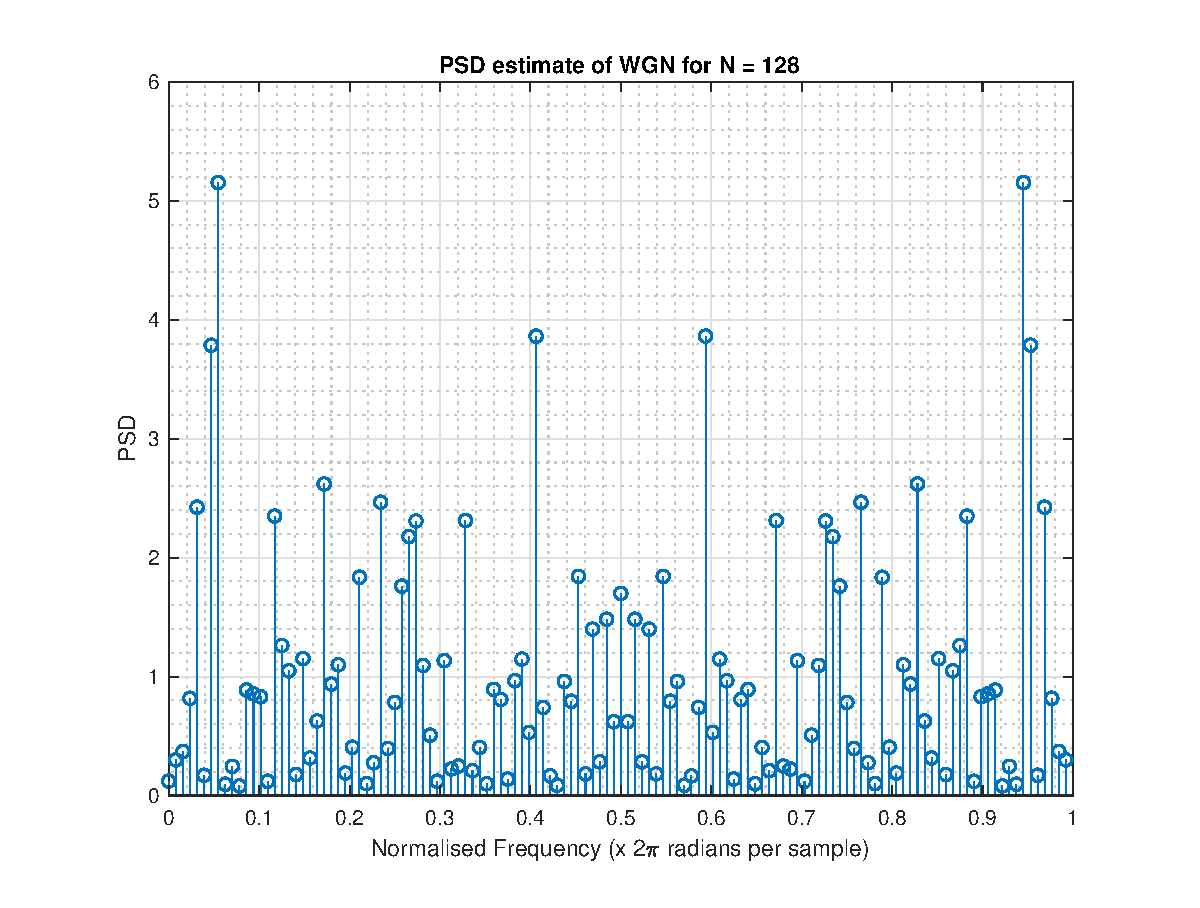
\includegraphics[width = \textwidth]{pgm_128}
\caption{N=128}
\label{fig:pgm_128}
\end{subfigure}
\begin{subfigure}{0.32\textwidth}
\centering
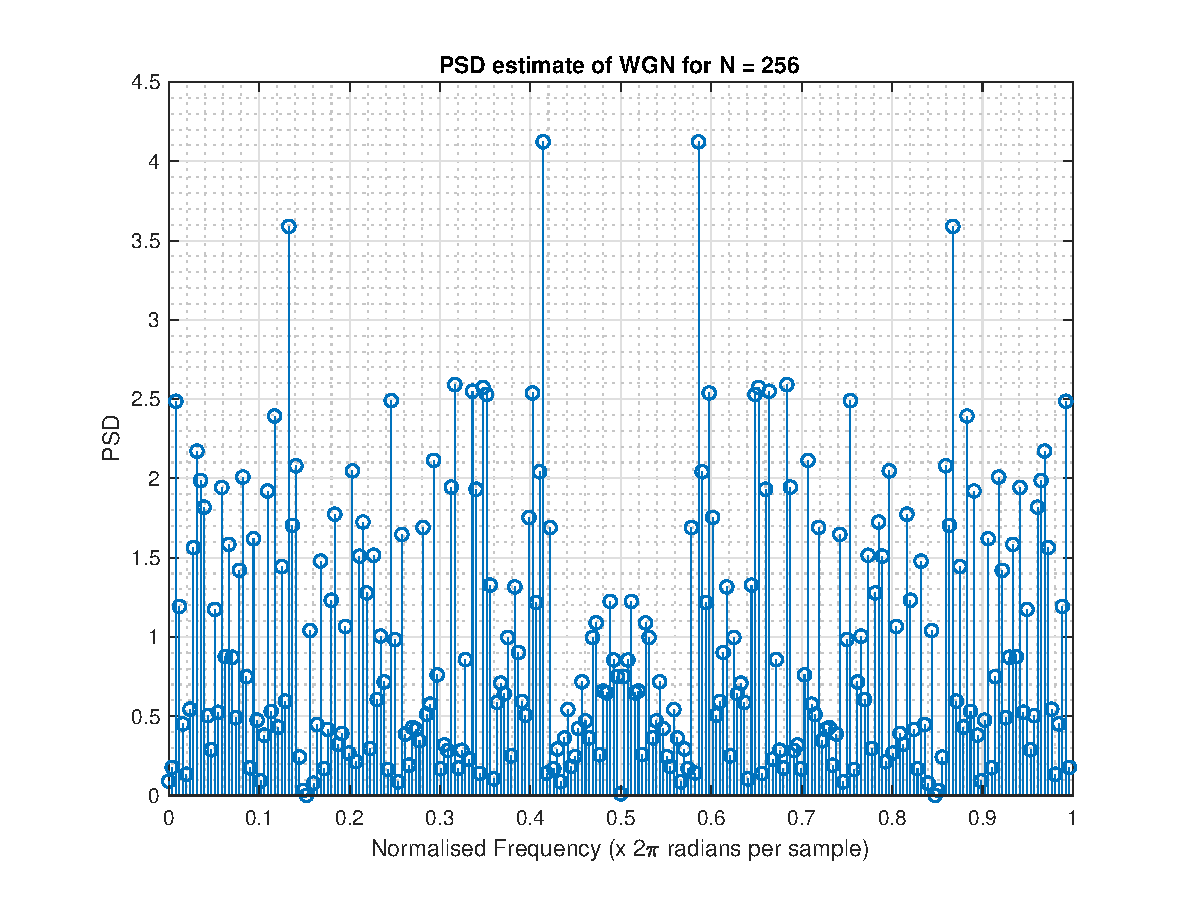
\includegraphics[width = \textwidth]{pgm_256}
\caption{N=256}
\label{fig:pgm_256}
\end{subfigure}
\begin{subfigure}{0.32\textwidth}
\centering
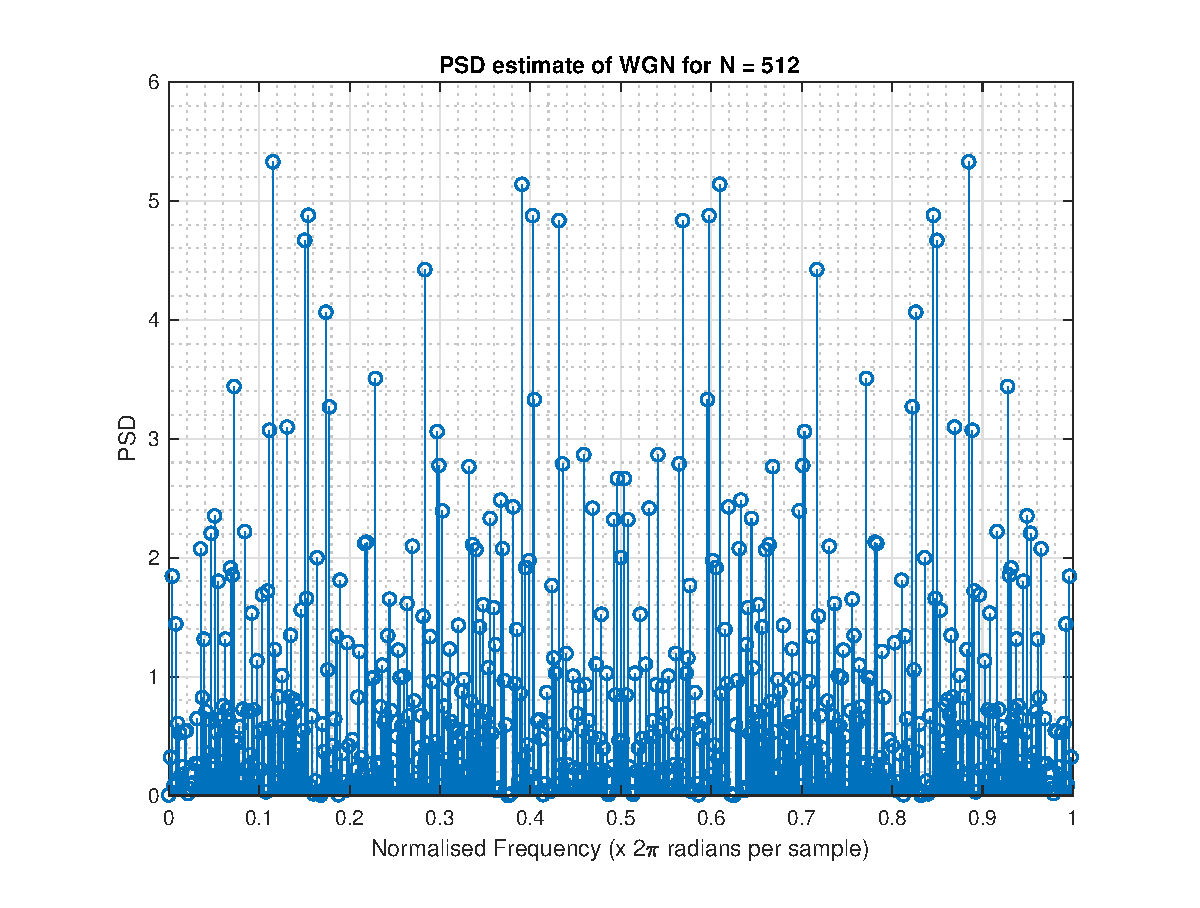
\includegraphics[width = \textwidth]{pgm_512}
\caption{N=512}
\label{fig:pgm_512}
\end{subfigure}
\caption{Estimated power spectral density for White Gaussian Noise}
\label{fig:pgm_test}
\end{figure}


\subsection{Averaged periodogram estimates}


\subsubsection{Smoothing the PSD estimate}

Smoothing creates an approximate function that retains important trends and patterns in the data while removing noise and other fine phenomena. While this reduces the variance of the data set, it decreases the resolution of frequency (0 to 0.5 instead of 0 to 1) and introduces a bias in the estimate. Figure \ref{fig:pgm_test_smooth} clearly shows that the smoothed estimate removes the large peaks from the original estimate.

\begin{figure}[h!]
\centering
\begin{subfigure}{0.32\textwidth}
\centering
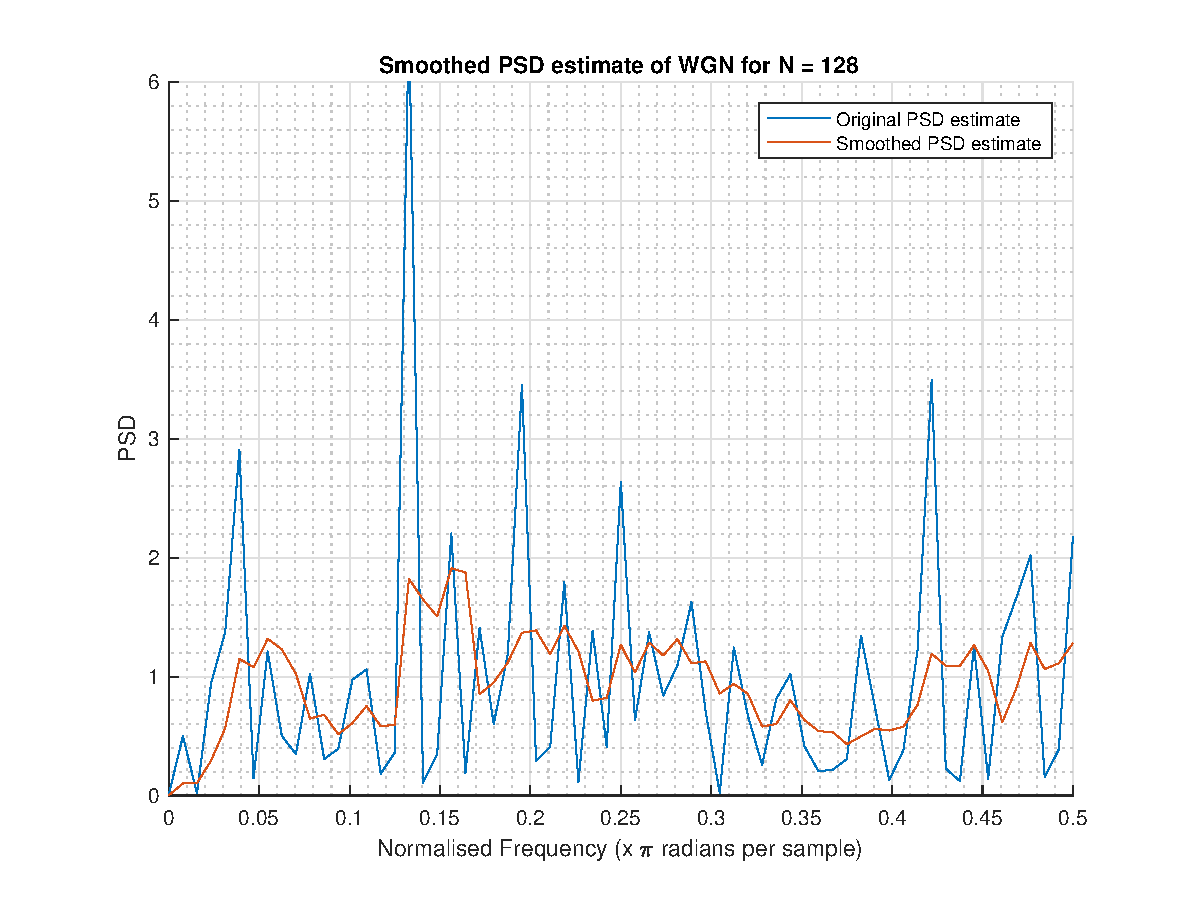
\includegraphics[width = \textwidth]{pgm_128_smooth}
\caption{N=128}
\label{fig:pgm_128_smooth}
\end{subfigure}
\begin{subfigure}{0.32\textwidth}
\centering
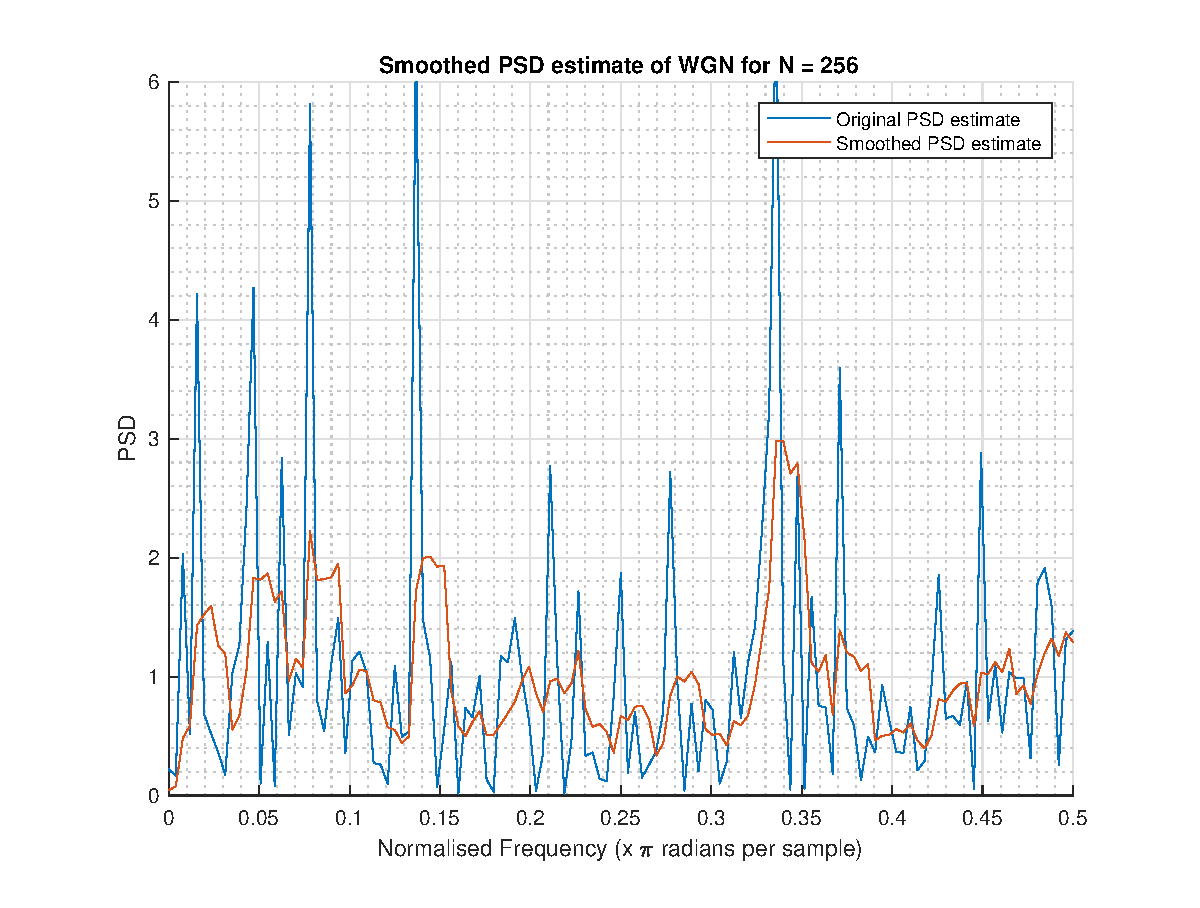
\includegraphics[width = \textwidth]{pgm_256_smooth}
\caption{N=256}
\label{fig:pgm_256_smooth}
\end{subfigure}
\begin{subfigure}{0.32\textwidth}
\centering
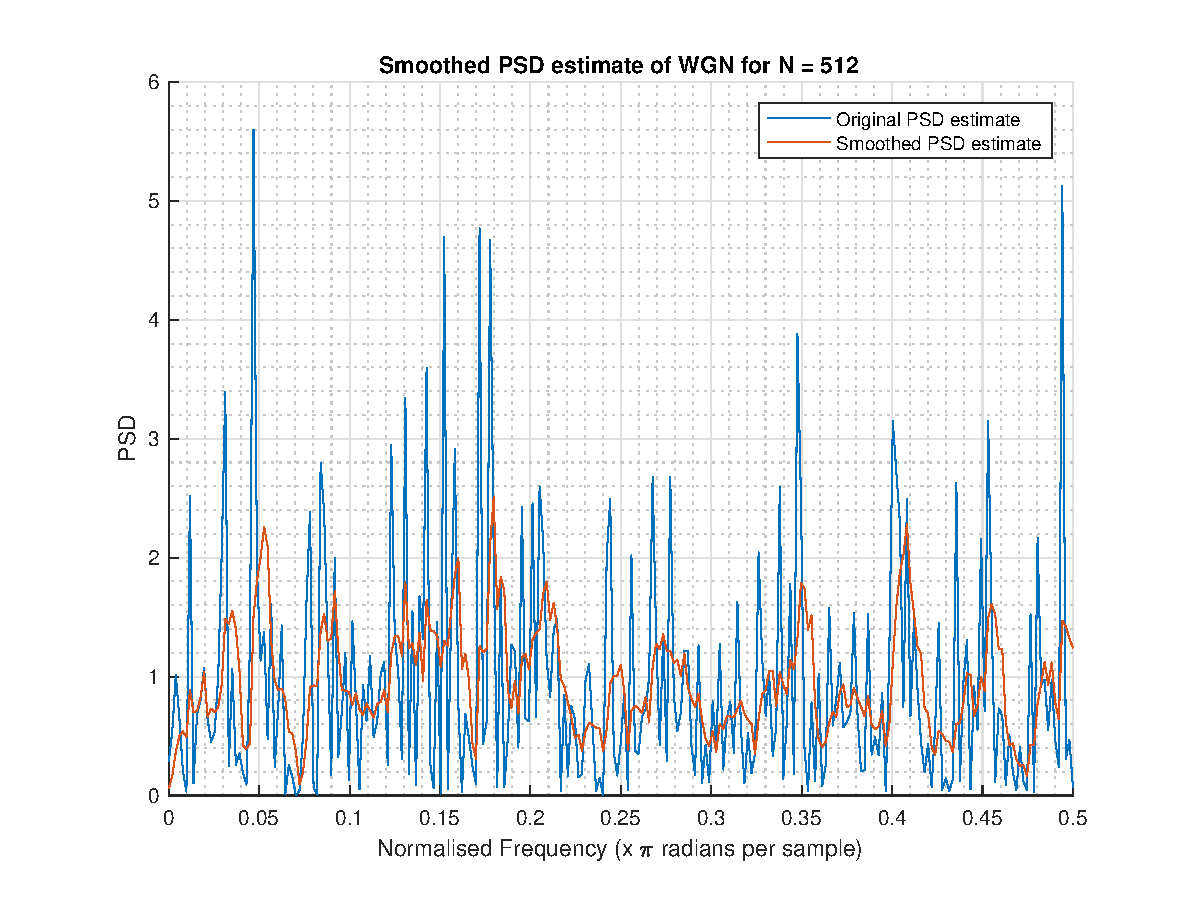
\includegraphics[width = \textwidth]{pgm_512_smooth}
\caption{N=512}
\label{fig:pgm_512_smooth}
\end{subfigure}
\caption{Smoothed estimated power spectral density for White Gaussian Noise}
\label{fig:pgm_test_smooth}
\end{figure}


\subsubsection{PSD estimates for non-overlapping WGN segments}

\begin{figure}[h!]
\centering
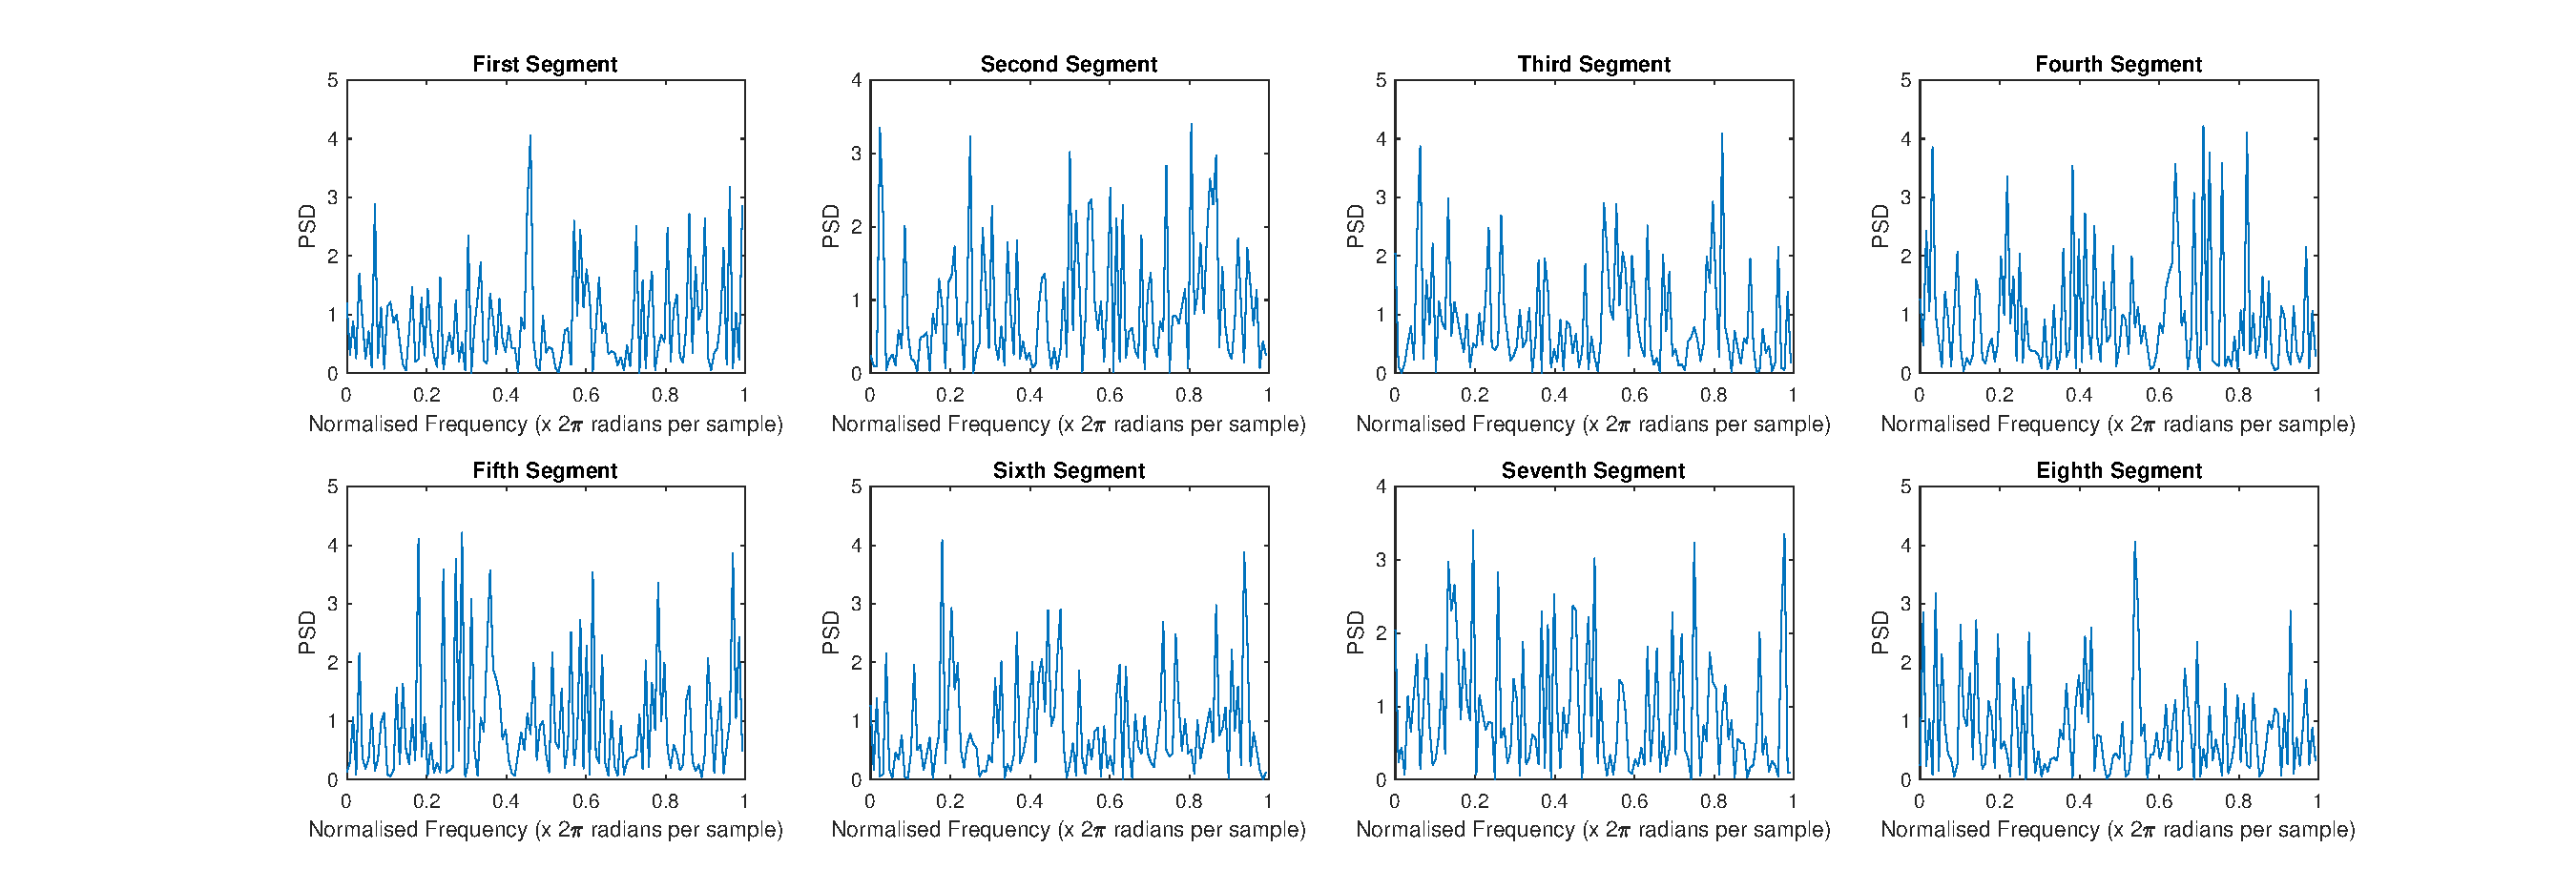
\includegraphics[width= \textwidth]{pgm_eightseg}
\caption{\label{fig:pgm_eightseg} PSD for 1024 samples split into 8 segments}
\end{figure}

The 8 non-overlapping segments are parts of a WGN signal and therefore completely random. The position of the peaks follows no pattern and their existence is attributed to the large variance of the data rather than a bias for specific frequencies. Thus each segment is an unreliable estimate for the ideal unity frequency PSD.


\subsubsection{Averaged Periodogram}

\begin{figure}[h!]
\centering
\begin{subfigure}{0.32\textwidth}
\centering
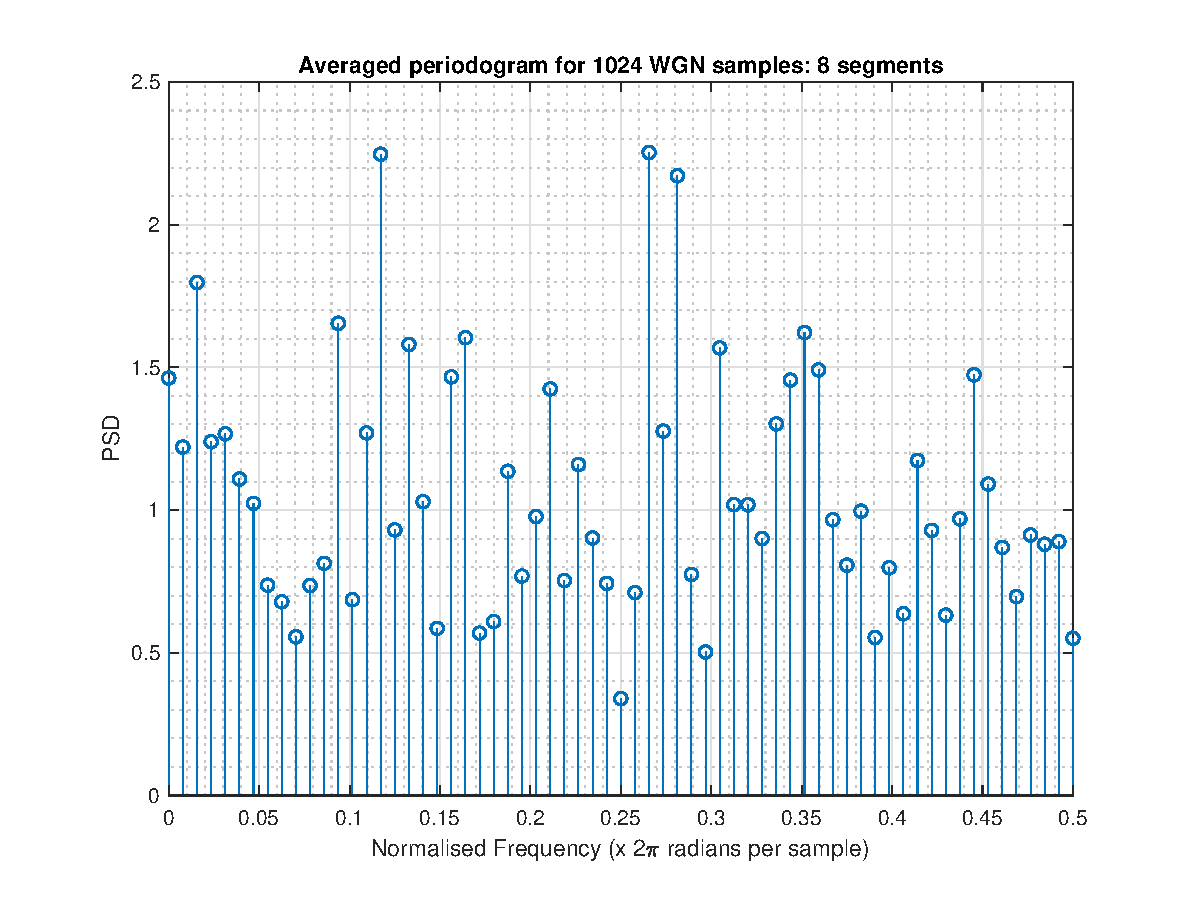
\includegraphics[width = \textwidth]{pgm_avg_8}
\caption{8 segments, 1024 samples}
\label{fig:pgm_avg_8}
\end{subfigure}
\begin{subfigure}{0.32\textwidth}
\centering
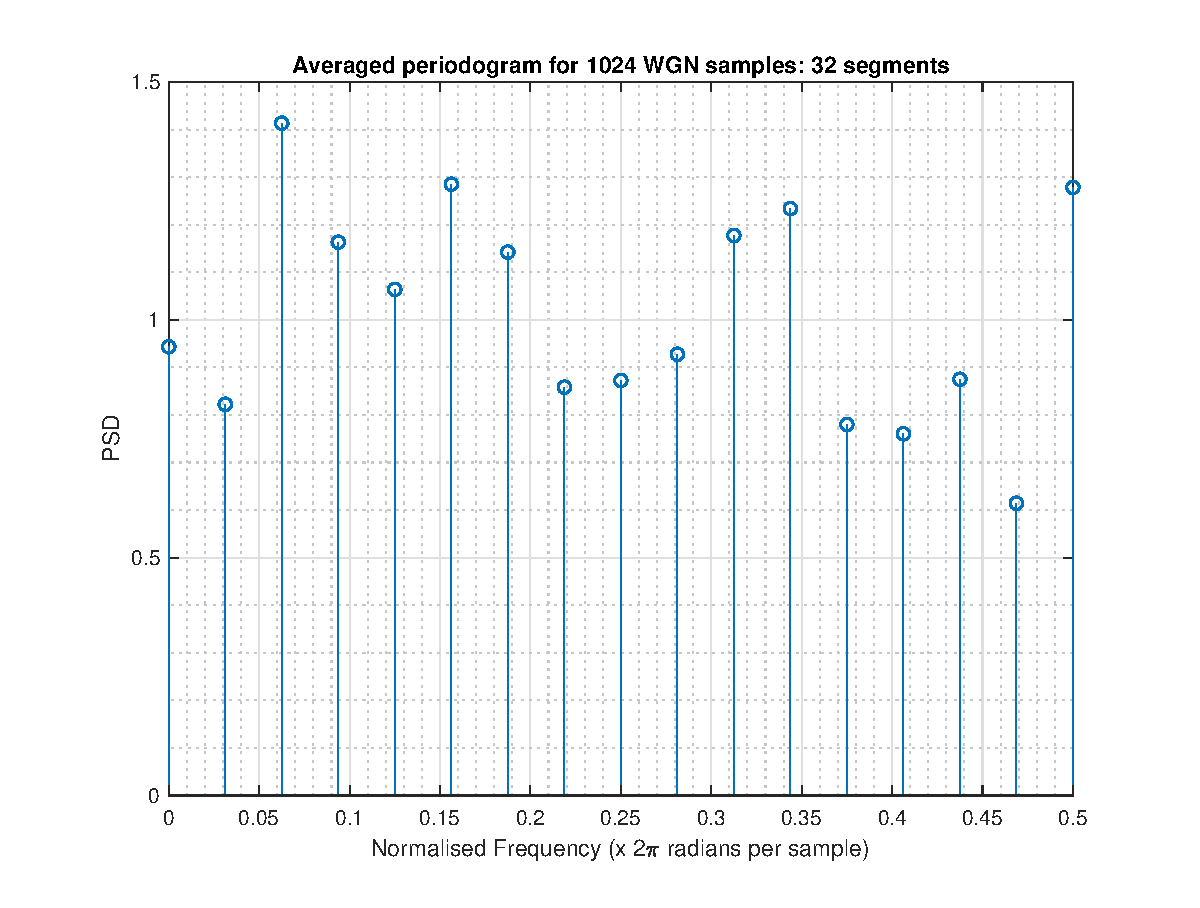
\includegraphics[width = \textwidth]{pgm_avg_32}
\caption{32 segments, 1024 samples}
\label{fig:pgm_avg_32}
\end{subfigure}
\begin{subfigure}{0.32\textwidth}
\centering
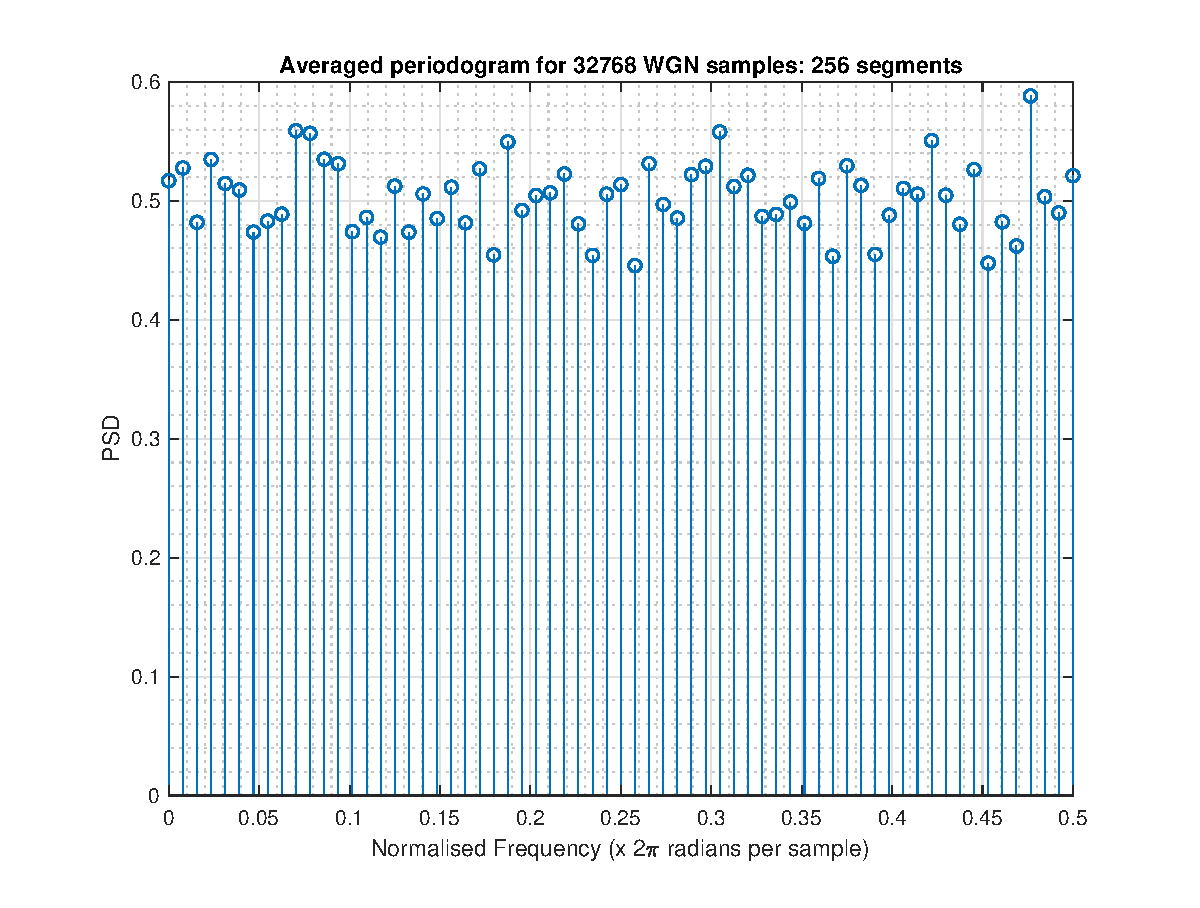
\includegraphics[width = \textwidth]{pgm_avg_256}
\caption{256 segments, 32768 samples}
\label{fig:pgm_avg_256}
\end{subfigure}
\caption{Averaged periodogram}
\label{fig: pgm_avg}
\end{figure}

Figure \ref{fig:pgm_avg_8} shows the average periodogram of 1024 WGN samples where averaging has been carried out in segment lengths of 8. Increasing the number of segments is linearly proportional to the decrease in variance, but we lose frequency resolution if the total number of samples is constant (shown in Figure \ref{fig:pgm_avg_32}). However, if we keep the samples per segment constant and simply increase the number of segments, we get a much more accurate estimate of the PSD (shown in Figure \ref{fig:pgm_avg_256}).


\subsection{Spectrum of autoregressive processes}

\begin{figure}[h!]
\centering
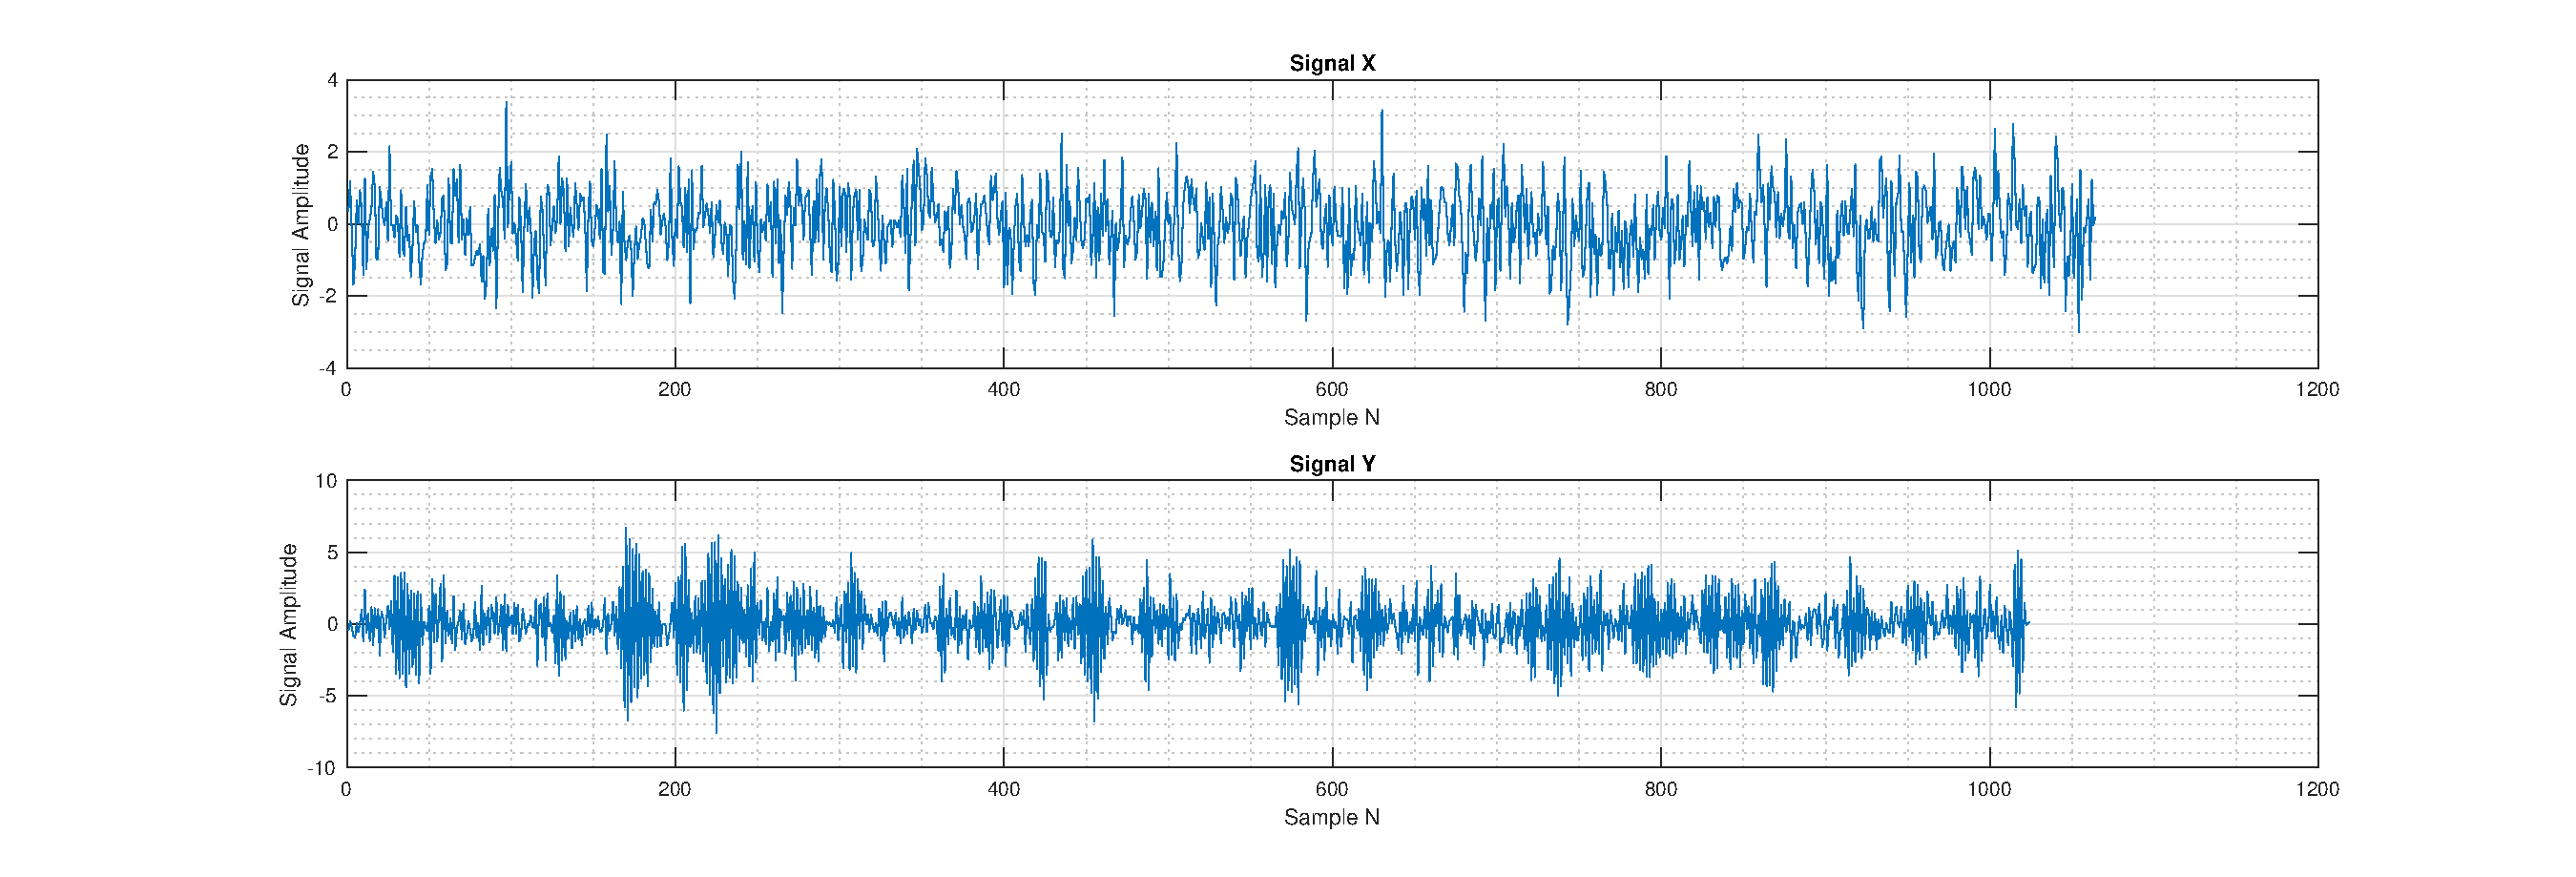
\includegraphics[width= \textwidth]{signals}
\caption{\label{fig:signals} Signals X and Y in time domain}
\end{figure}

We can see in Figure \ref{fig:signals} that the WGN sequence \textbf{x} has been high pass filtered into \textbf{y} since the filter has attenuated the low frequency elements and left the high frequency components.

\begin{figure}[h!]
\centering
\begin{subfigure}{0.32\textwidth}
\centering
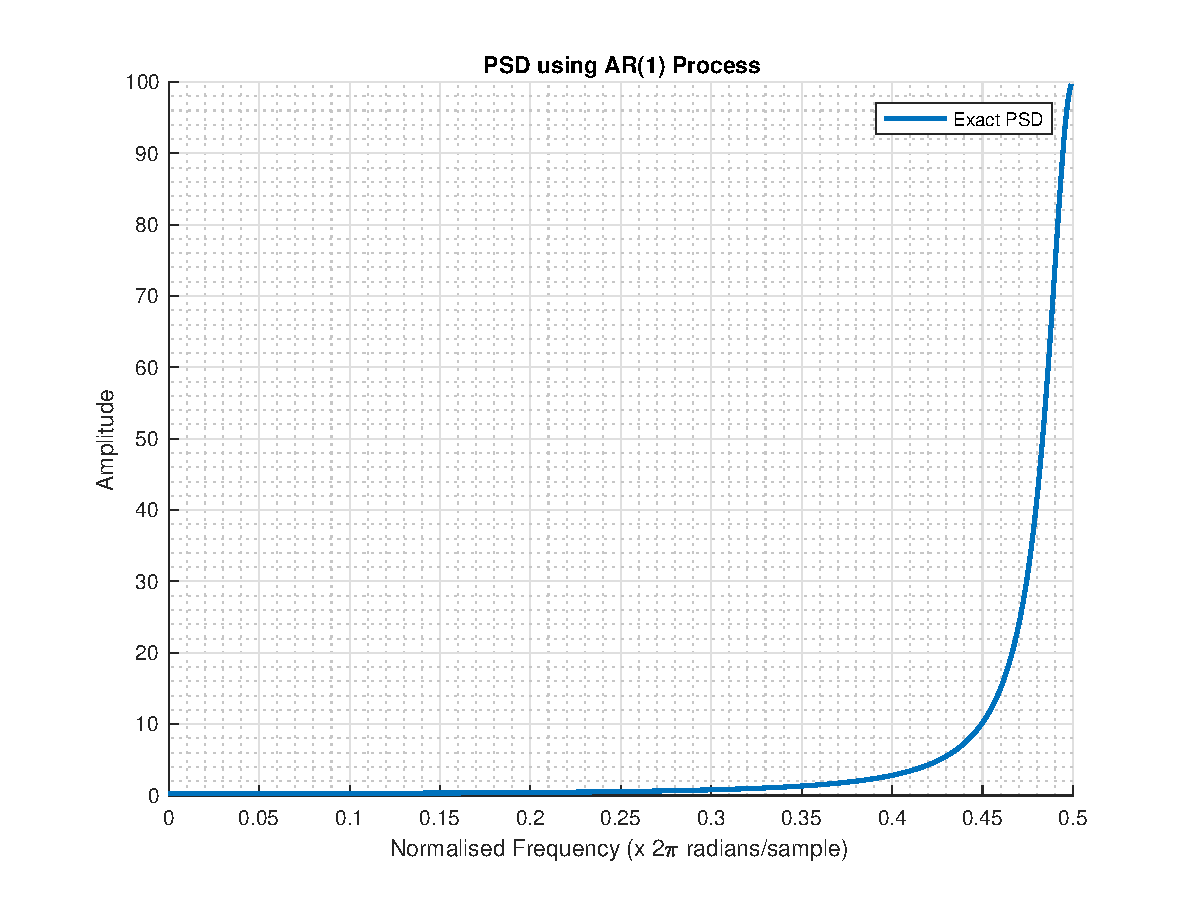
\includegraphics[width = \textwidth]{ar1_psd_exact}
\caption{Ideal PSD response}
\label{fig:ar1_psd_exact}
\end{subfigure}
\begin{subfigure}{0.32\textwidth}
\centering
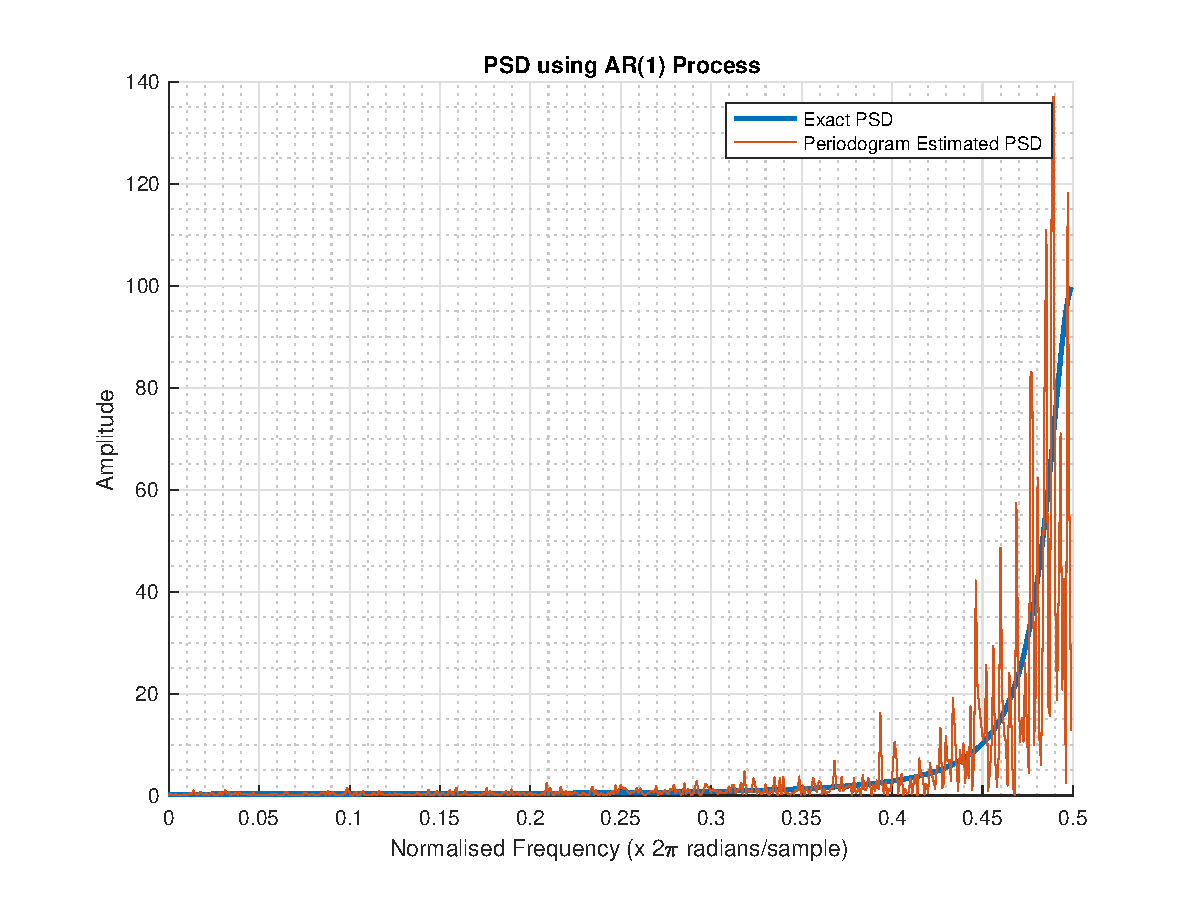
\includegraphics[width = \textwidth]{ar1_psd_est}
\caption{Ideal and estimated PSD}
\label{fig:ar1_psd_est}
\end{subfigure}
\begin{subfigure}{0.32\textwidth}
\centering
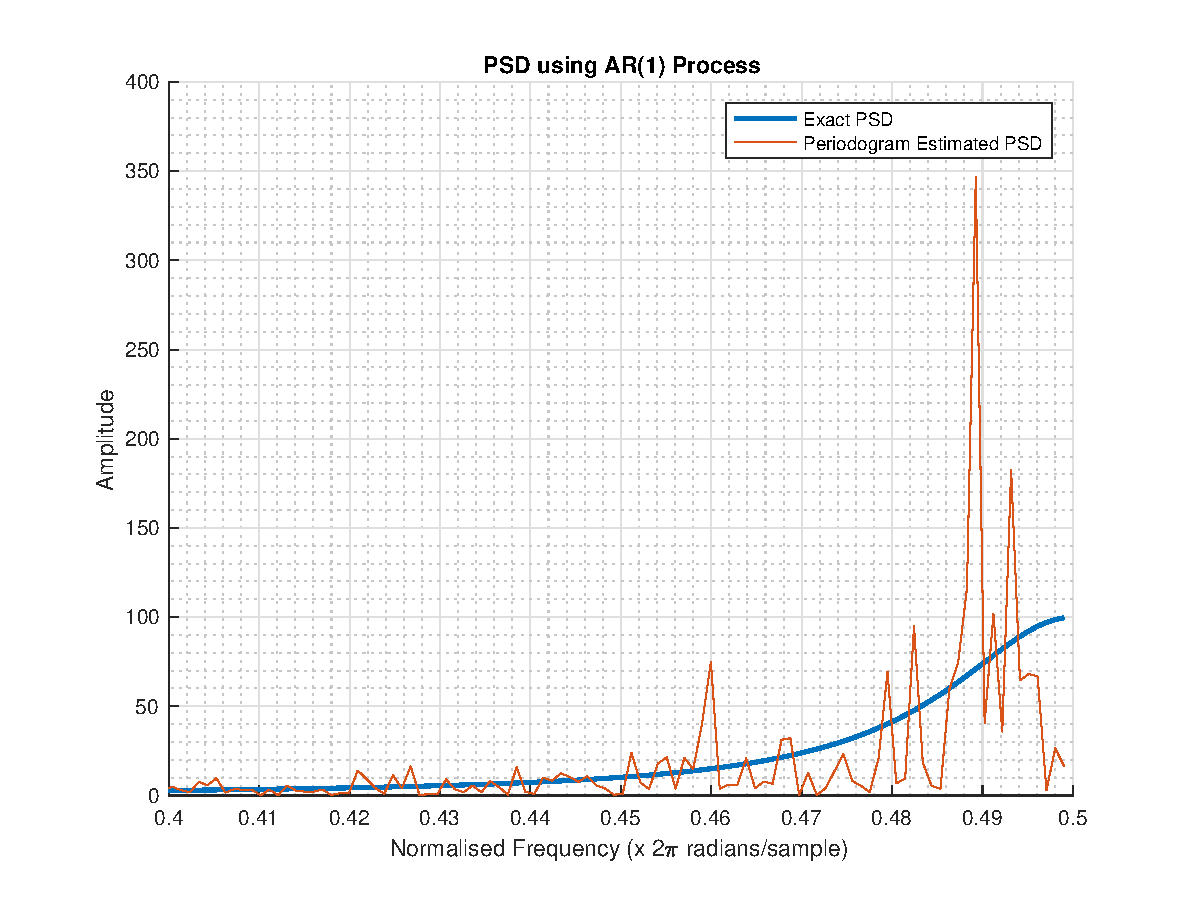
\includegraphics[width = \textwidth]{ar1_psd_est_zoom}
\caption{Windowing f = 0.4 - 0.5}
\label{fig:ar1_psd_est_zoom}
\end{subfigure}
\caption{Ideal PSD, periodogram estimate of PSD, and windowing the PSD}
\label{fig:ar_spec}
\end{figure}


\subsubsection{Ideal PSD response}

Figure \ref{fig:ar1_psd_exact} shows the exact PSD of the output signal \textbf{y}. The normalized cut-off frequency is approximately 0.39 Hz and the maximum PSD value is at 0.5 Hz. Note that the plots in Figure \ref{fig:ar_spec} have been shown only up to f = 0.5 Hz since the figures will be symmetric about f = 0.5 Hz.

\subsubsection{Periodogram estimate of PSD response}

The periodogram estimate is based on a finite number of samples and hence has some error in its estimation. However, the periodogram successfully suppresses lower frequencies and allows high frequencies to pass.

\subsubsection{Effect of windowing}

The finite length from 0.4 to 0.5 is obtained by multiplying the long signal by a window in the time domain, which corresponds to convolution with a sinc function in the frequency domain.

\begin{equation*}
\mathcal{F}_{rect(\frac{t}{a})}(f)=a \cdot sinc(af)
\end{equation*}

This has an insignificant effect at lower frequencies where the PSD is almost 0 but distorts the PSD at higher frequencies.

\subsubsection{Model based PSD}

\begin{figure}[h!]
\centering
\begin{subfigure}{0.32\textwidth}
\centering
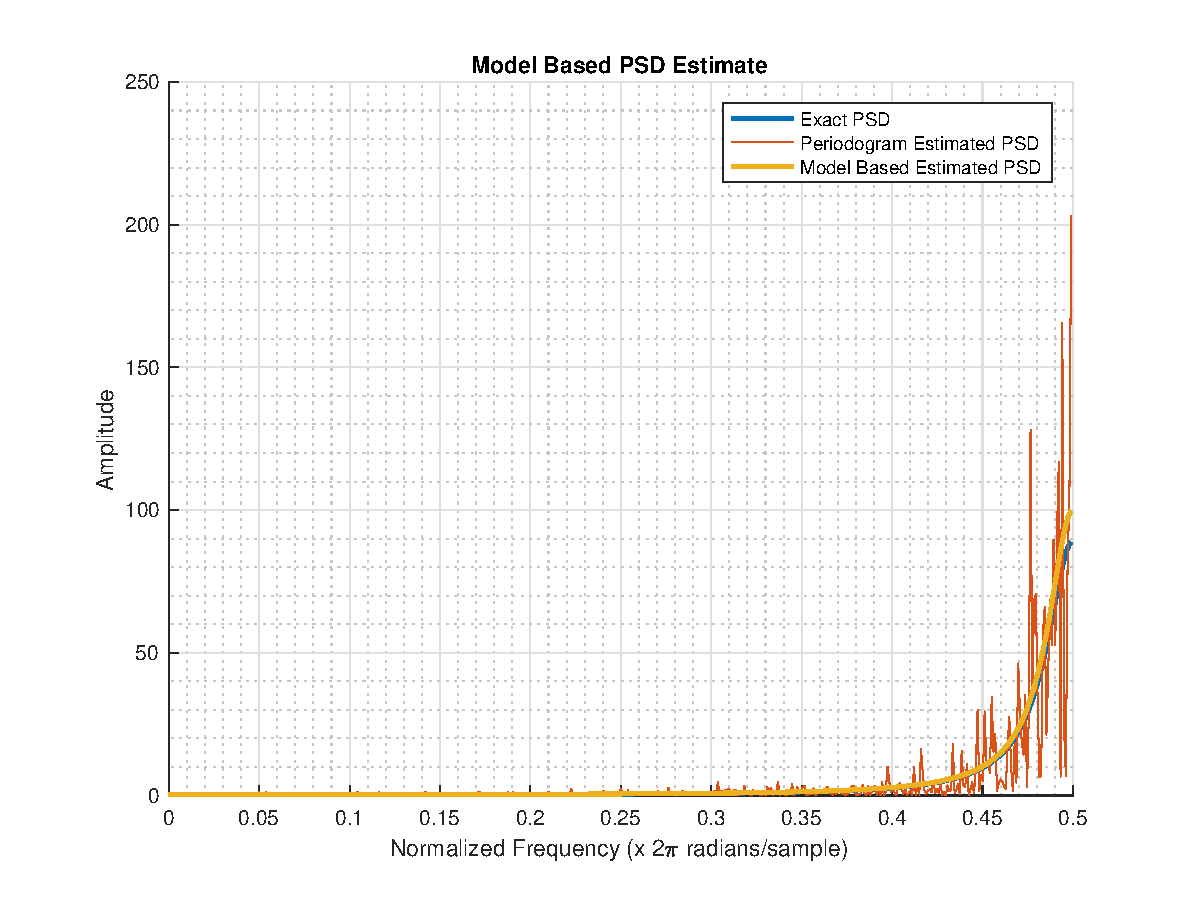
\includegraphics[width = \textwidth]{ar_spec_model}
\caption{Ideal and estimated PSD}
\label{fig:ar_spec_model}
\end{subfigure}
\begin{subfigure}{0.32\textwidth}
\centering
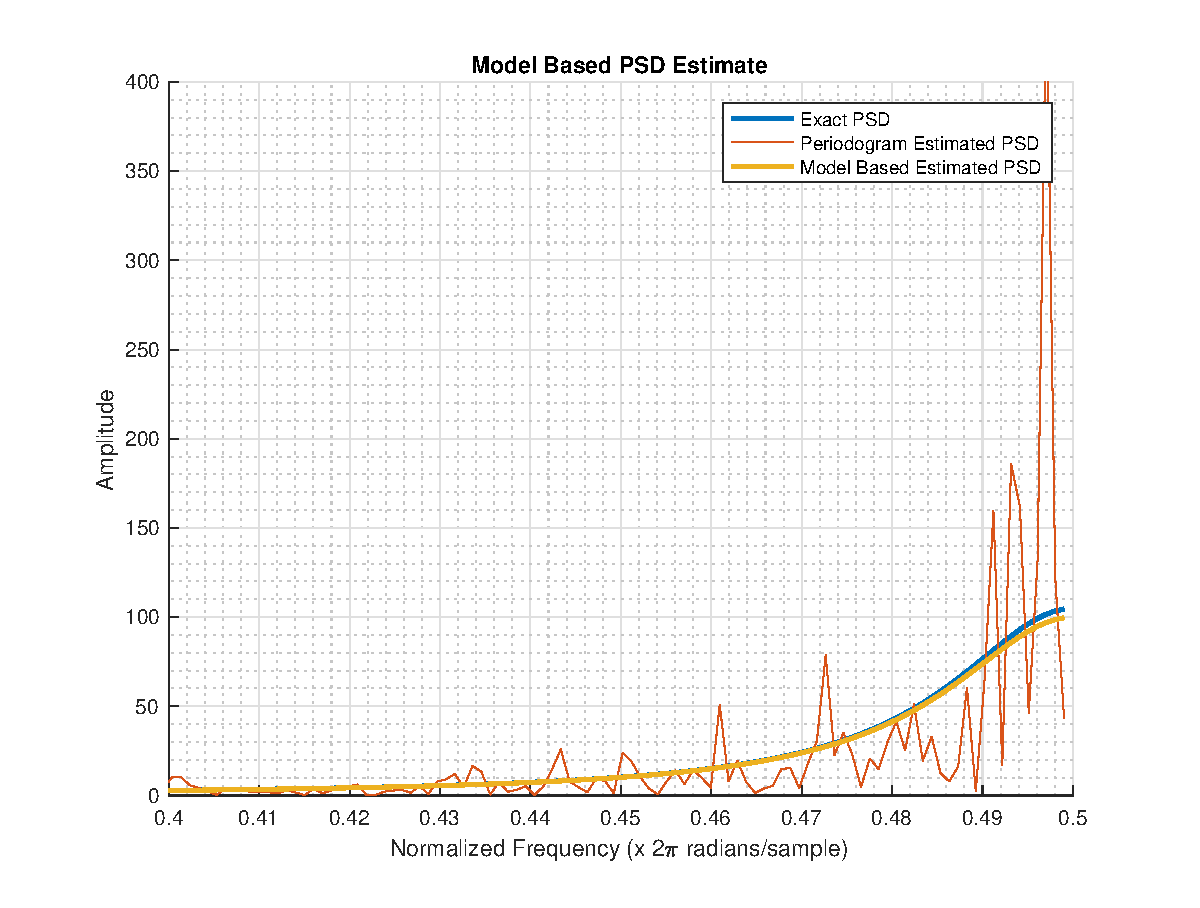
\includegraphics[width = \textwidth]{ar_spec_model_zoom}
\caption{Windowing f = 0.4 - 0.5}
\label{fig:ar_spec_model_zoom}
\end{subfigure}
\caption{Comparing the PSD estimate of the model based method and the periodogram}
\label{fig:ar_spec_modvpgm}
\end{figure}

Since we have seen how unreliable the periodogram is, we now explicitly model the signal as an AR(1) process defined by $a_1$ and $\sigma_x^2$. This approach caters to the specific type of data we are using and hence is more accurate than the periodogram which uses the same approach for every data type. It is also immune to the error introduced because of the convolution with the sinc function due to windowing.

\pagebreak

\subsubsection{Application to sunspot time series}

\begin{figure}[h!]
\centering
\begin{subfigure}{0.32\textwidth}
\centering
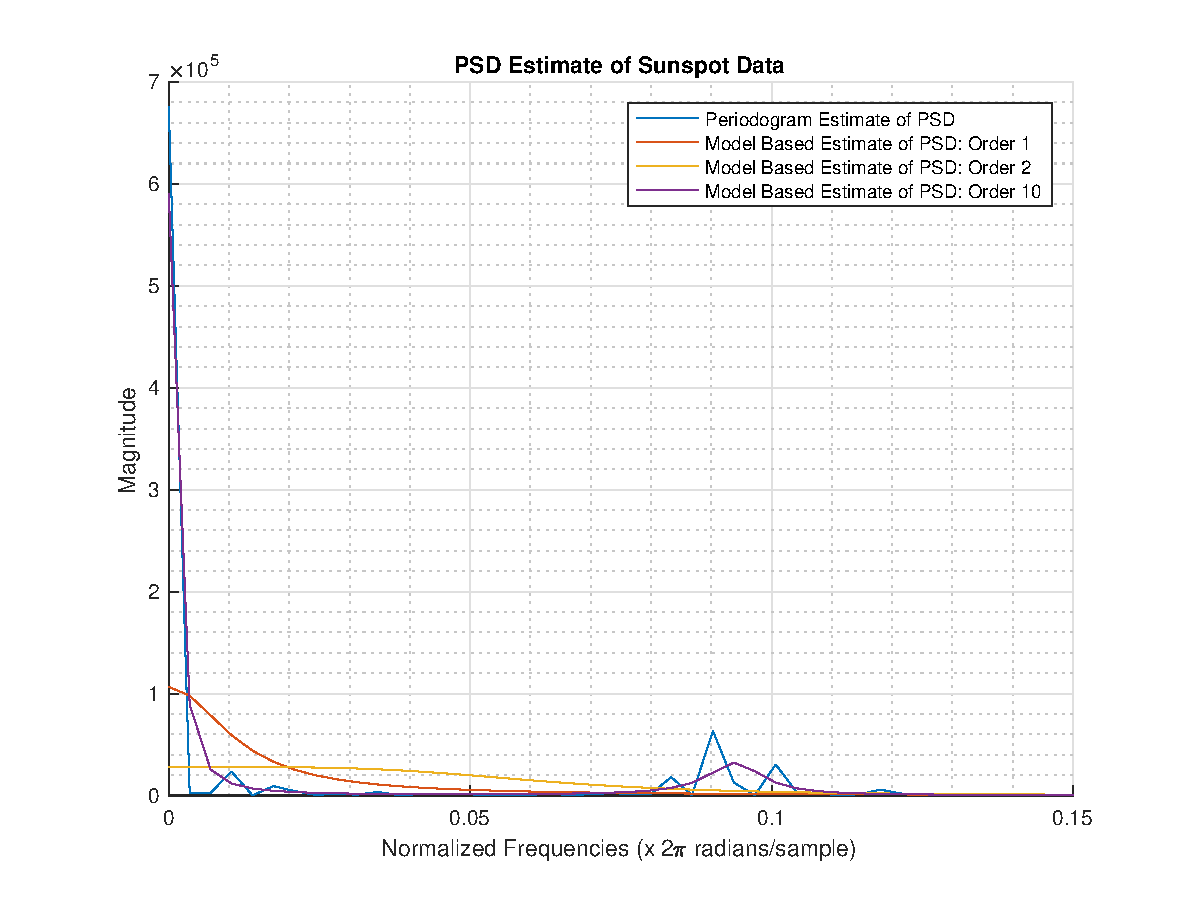
\includegraphics[width = \textwidth]{ar_model_sunspot_orig}
\caption{Original Data}
\label{fig:ar_model_sunspot_orig}
\end{subfigure}
\begin{subfigure}{0.32\textwidth}
\centering
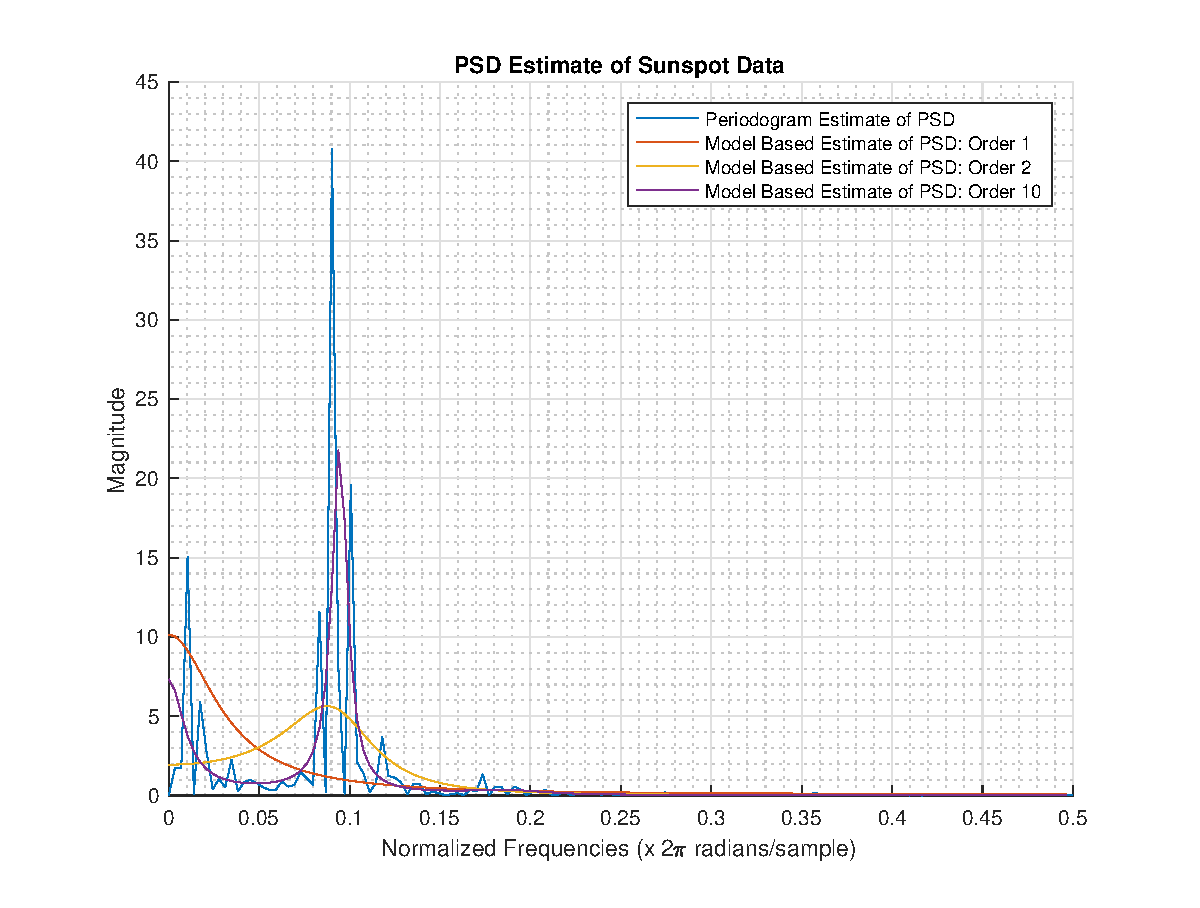
\includegraphics[width = \textwidth]{ar_model_sunspot}
\caption{Normalized Data}
\label{fig:ar_model_sunspot}
\end{subfigure}
\begin{subfigure}{0.32\textwidth}
\centering
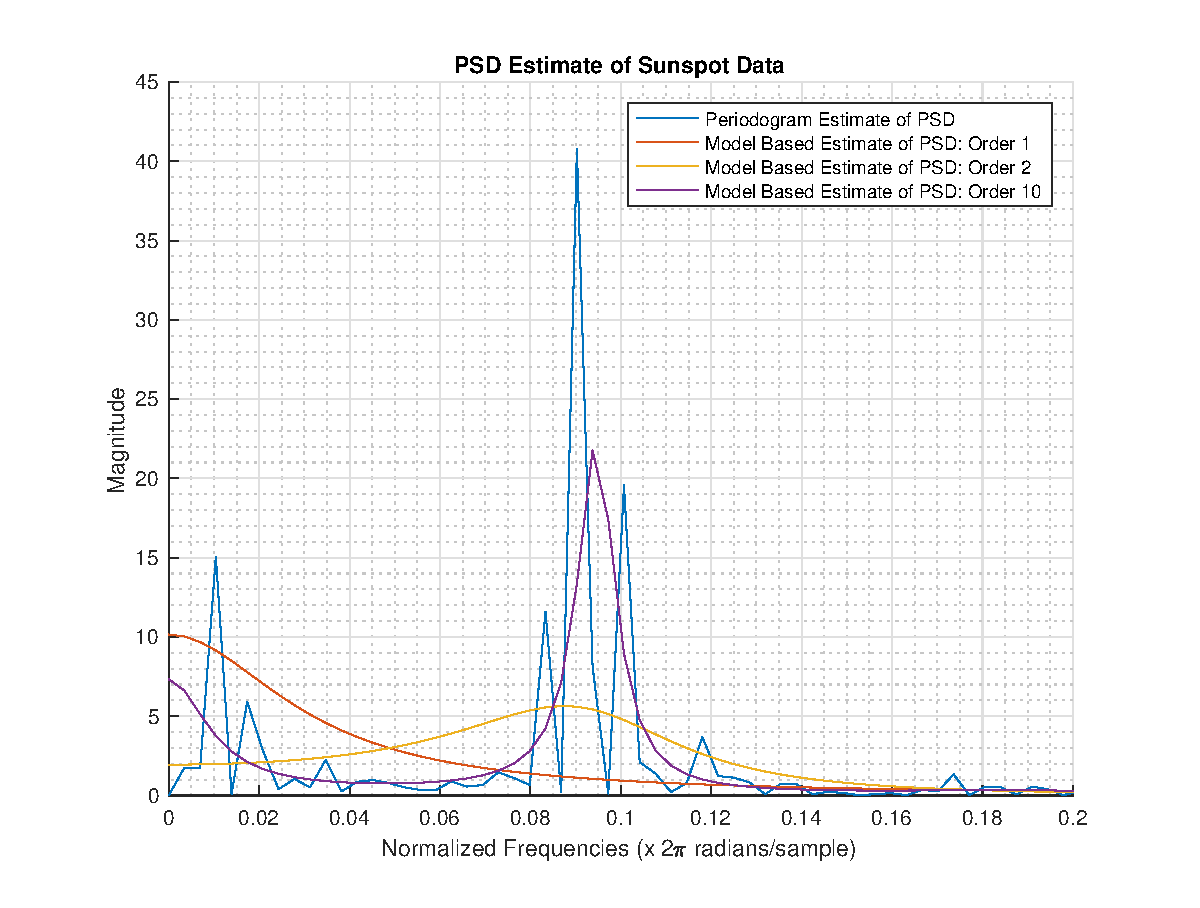
\includegraphics[width = \textwidth]{ar_model_sunspot_zoom}
\caption{Windowing f = 0 - 0.2}
\label{fig:ar_model_sunspot_zoom}
\end{subfigure}
\caption{PSD estimate using the model based method and the periodogram for sunspot data}
\label{fig:ar_spec_sunspot}
\end{figure}

We know from our earlier analysis using the MDL and AIC that the optimal order for modeling the sunspot data is 2. Order 1 is not flexible enough to show the periodicity properly and order 10 is more accurate but computationally more complex. AR(2) strikes the right balance, while AR(1) under-models the data and AR(10) over-models it.


\subsection{The Least Squares Estimation (LSE) of AR Coefficients}

\subsubsection{General Form of Cost Function}

An autoregressive moving average (ARMA) model assumes a PSD of:

\begin{equation}
P_{xx}(f) = \frac{\sigma_u^2|B(f)|^2}{|A(f)|^2}
\end{equation}

where

\begin{align}
B(f) &= 1 + \sum_{k=1}^q {b[k] exp(-j2\pi fk)} \\
A(f) &= 1 + \sum_{k=1}^p {a[k] exp(-j2\pi fk)}
\end{align}
\\
Here the b[k] terms are the MA filter parameters and the a[k] terms are the AR filter parameters. The LSE approach only focuses on the AR parameters. We now take the inverse z transform of the PSD to find the ACF:

\begin{equation}
P_{xx}(z) = \frac{\sigma^2 B(z)B(z^{-1})}{A(z)A(z^{-1})}
\end{equation}
\\
where $B(f)=B(exp(j2\pi f))$ and $A(f)=A(exp(j2\pi f))$.

\begin{equation}
Z^{-1}[A(z)P_{xx}(z)] = Z^{-1} [\sigma^2 \frac{B(z^{-1})}{A(z)^{-1}}]
\end{equation}

Since the filter impulse response is causal,

\begin{align}
h[n] &= Z^{-1} \frac{B(z)}{A(z)} = 0 \text{ for }n<0 \\
\text{and }h[-n] &= Z^{-1} \frac{B(z^{-1})}{A(z^{-1})} = 0 \text{ for }n>0
\end{align}

Thus the system is anticausal and we have:

\begin{equation}
Z^{-1} {\sigma^2 B(z) \frac{B(z^{-1})}{A(z^{-1})}} = \sigma^2 b[n] \times h[-n]
\end{equation}

\begin{equation}
Z^{-1} {\sigma^2 B(z) \frac{B(z^{-1})}{A(z^{-1})}} = 
\begin{cases}
\sigma^2 b[n] \times h[-n] \star h[-n] \\
0, & n>q
\end{cases}
\end{equation}

\begin{equation}
\therefore Z^{-1}[A(z)P_{xx}(z)] = Z^{-1} [{\sigma^2 B(z) \frac{B(z^{-1})}{A(z^{-1})}}] = 0 \text{ for }n>q
\end{equation}

The difference equation of the ACF for $n>q$ can now be written as:

\begin{equation}
\sum_{k=0}^p {a[k]r_{xx}[n-k]=0} \text{ for } n>q
\end{equation}
\\
where a[0]=1. These equations are known as the modified Yule Walker equations since they are identical to the original Yule Walker equations except for the fact that they hold for $n>0$. Assuming x[n] is available from 0,1,...(N-1), and the ACF is estimated for lags n = 0,1,...M, where $M <= N-1$, then the LSE of a[k] will minimize:

\begin{align}
J &= \sum_{n=q+1}^M {[ \hat{r_{xx}}[n] - ( - \sum_{k=1}^p a[k] \hat{r_{xx}}[n-k])]^2} \\
&= (x - H\theta)^T (x - H\theta)
\end{align}

where

\begin{equation}
x = 
\begin{bmatrix}
\hat{r_{xx}[q+1]}\\
\hat{r_{xx}[q+2]}\\
\vdots
\hat{r_{xx}[M]}
\end{bmatrix}
\end{equation}

\begin{equation}
\theta = 
\begin{bmatrix}
a[1]\\
a[2]\\
\vdots
a[p]
\end{bmatrix}
\end{equation}

\begin{equation}
H = 
\begin{bmatrix}
\hat{r_{xx}}[q] & \hat{r_{xx}}[q-1] & \cdots & \hat{r_{xx}}[q-p+1]\\
\hat{r_{xx}}[q+1] & \hat{r_{xx}}[q] & \cdots & \hat{r_{xx}}[q-p+2]\\
\vdots & \vdots & \vdots & \vdots\\
\hat{r_{xx}}[M] & \hat{r_{xx}}[M-2] & \cdots & \hat{r_{xx}}[M-p]
\end{bmatrix}
\end{equation}
\\

\subsubsection{Examining the observation matrix H}
\vspace{0.5cm}

\begin{equation}
LSE_{\theta} = (H^TH)^{-1}H^Tx
\end{equation}
\\
This is termed as the least squares modified Yule Walker equations, where the LSE is being used for the ACF estimate instead of actual data. While the observation matrix H is usually deterministic, it is now completely random. M should be small since the estimate is prone to higher error at larger lags due to the averaging of (N-k) products in the calculation of $r_{xx}[k]$.

\pagebreak % NEED TO FINISH!!


\subsection{Spectrogram for time frequency analysis: Dial tone pad}

\subsubsection{The London land-line number}

A random London land-line number of the form 020 XXXX XXXX is generated, and the signal for the first 2 digits (blank included) is shown in Figure \ref{fig:dtp_2dig}. The number used for all the following analysis is 02044081677.

\begin{figure}[h!]
\centering
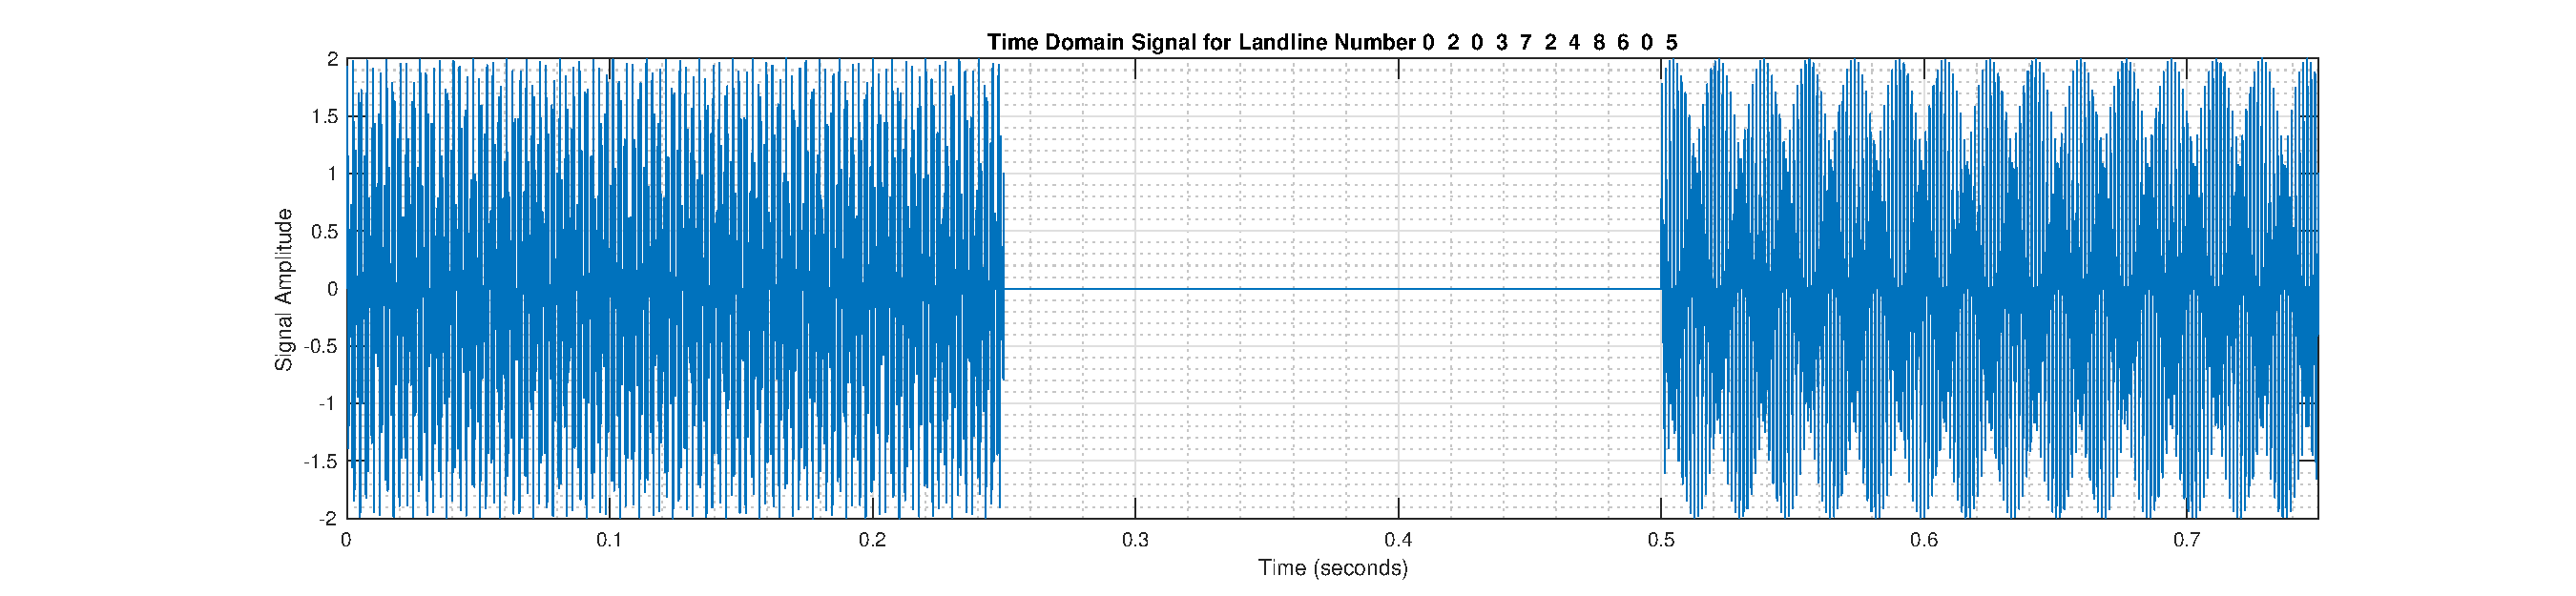
\includegraphics[width= 0.8\textwidth]{dtp_2dig}
\caption{\label{fig:dtp_2dig} Signal for 0 and 2 separated by a blank}
\end{figure}

The minimum sampling frequency (Nyquist frequency) must be 2954 Hz since the maximum frequency on the given look up table is 1477 Hz. A sampling frequency of 32768 Hz ensures that there will be no aliasing for signals up to 16384 Hz, which is well above our requirement. Sampling at a higher frequency than what is required gives more effective number of bits (ENOB) which helps boost the SNR.

\subsubsection{Analyzing the spectrogram}

\begin{figure}[h!]
\centering
\begin{subfigure}{0.32\textwidth}
\centering
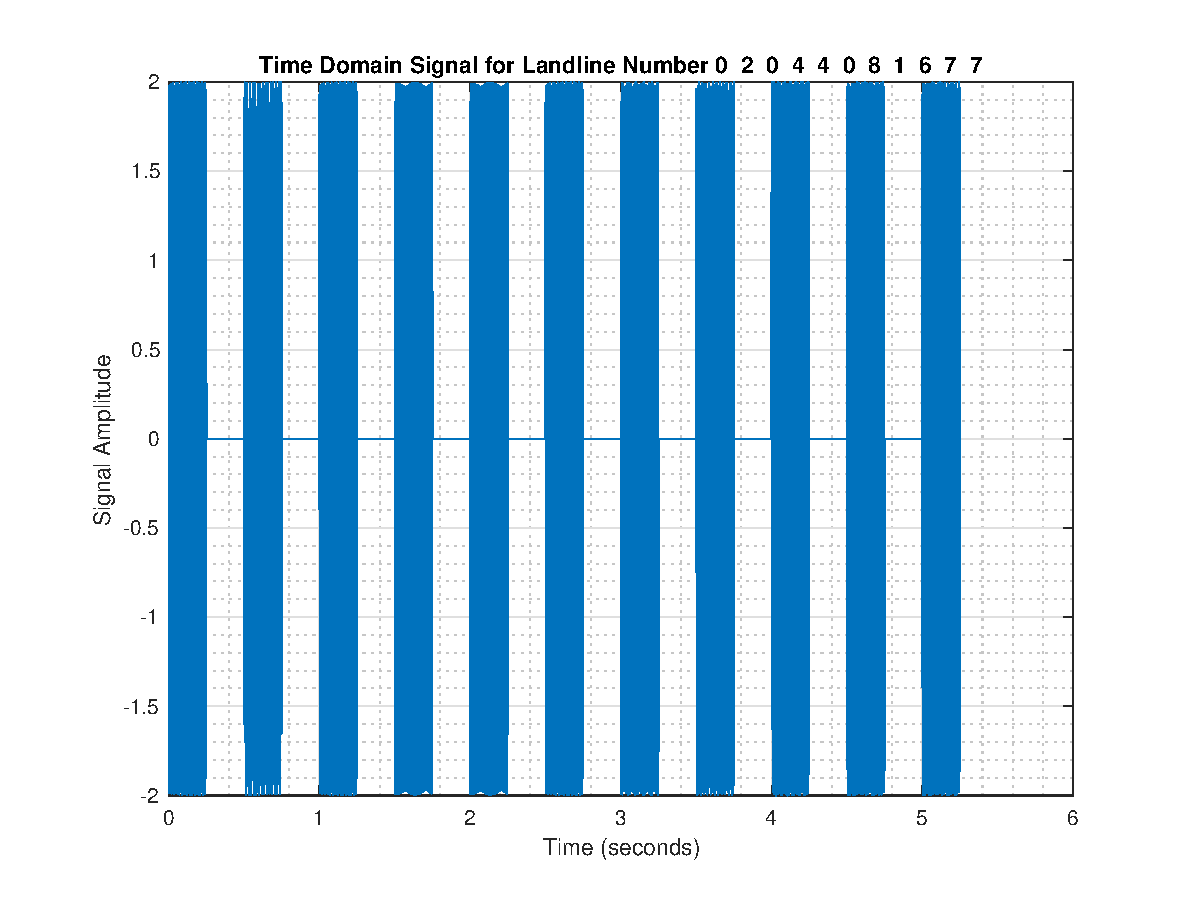
\includegraphics[width = \textwidth]{dtp_fullsig}
\caption{Full time domain signal}
\label{fig:dtp_fullsig}
\end{subfigure}
\begin{subfigure}{0.32\textwidth}
\centering
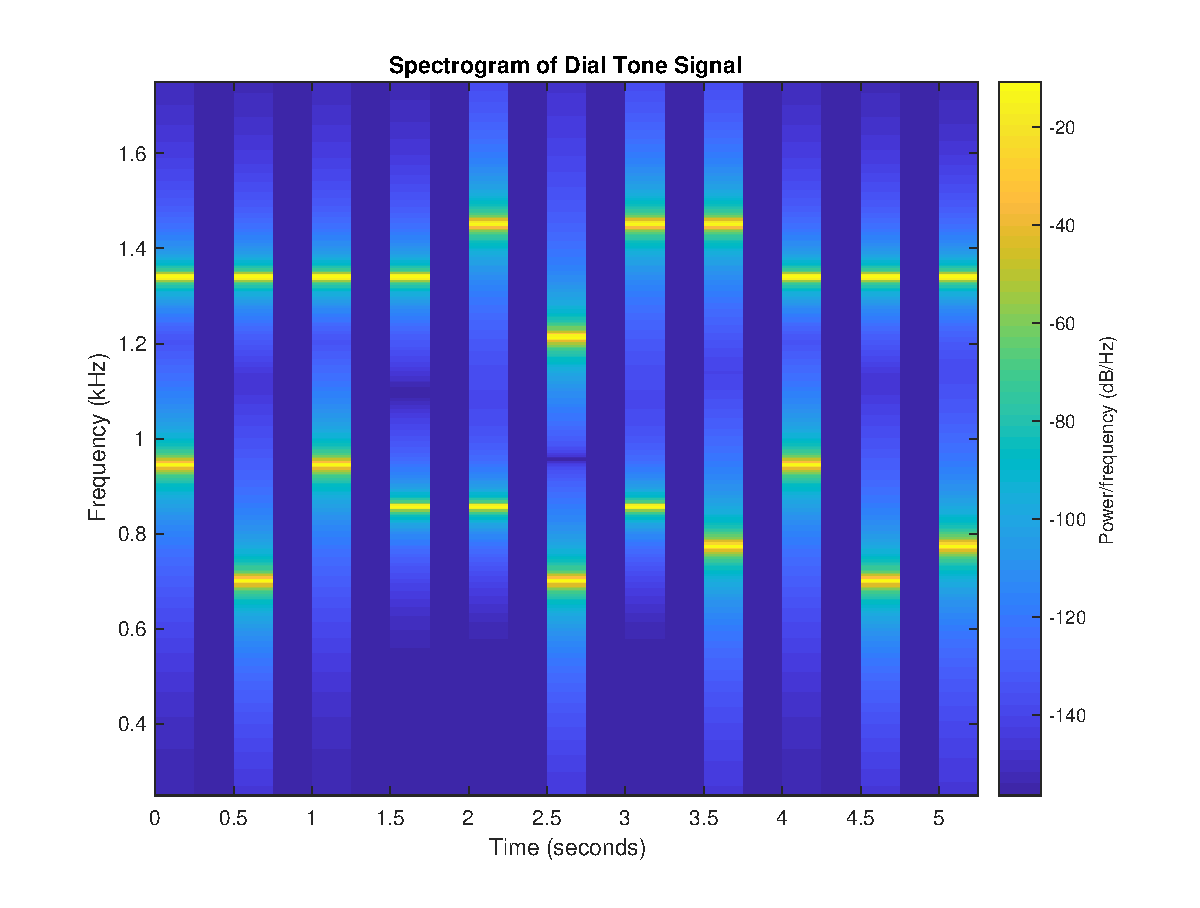
\includegraphics[width = \textwidth]{dtp_spectrogram}
\caption{Full spectrogram}
\label{fig:dtp_spectrogram}
\end{subfigure}
\begin{subfigure}{0.32\textwidth}
\centering
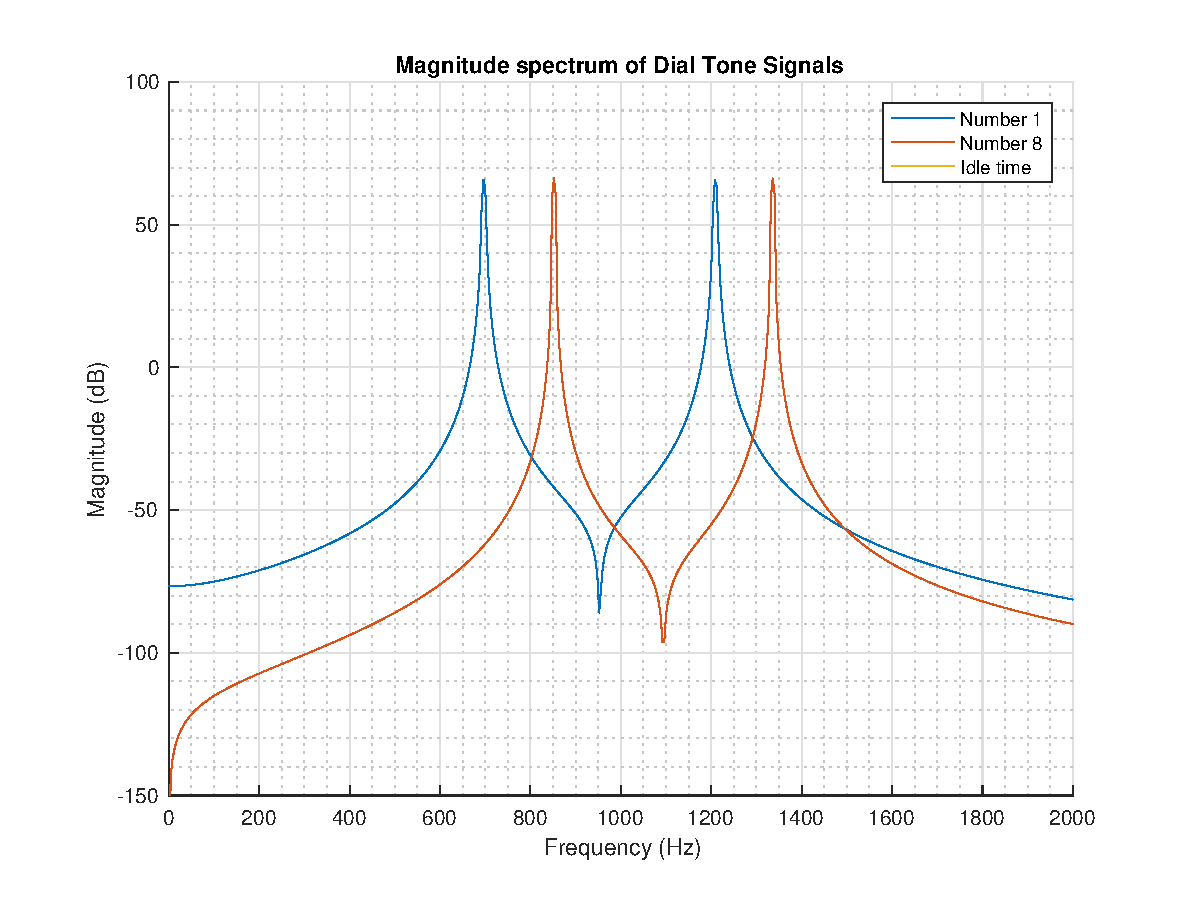
\includegraphics[width = \textwidth]{dtp_magspec}
\caption{Power for digits 1 \& 8}
\label{fig:dtp_magspec}
\end{subfigure}
\caption{The spectrogram shows how the signal's power varies with time and frequency}
\label{fig:ar_spec_sunspot}
\end{figure}

The spectrogram in Figure \ref{fig:dtp_spectrogram} clearly shows the power peaks at specific frequencies for each key as time passes. The vertical variation (power vs frequency) is further examined in Figure \ref{fig:dtp_magspec} where we can see two distinct peaks for numbers 1 and 8. Note that there is no idle time signal here since we have not introduced any noise yet.\\

The spreading of the spectrum in the spectrogram is due to the side lobes introduced by the Hanning window. Since we need 32768 samples per second, and each key has a duration of 0.25 seconds, we split each key's spectrum into 8192 samples. This is a finite number, and hence leads to a slight displacement in the position of the peaks from the ideal.

\subsubsection{Key Classification}

We can examine each block of 8192 samples separately to identify the two frequency peaks for the key pressed. Allowing for some tolerance from the maximum and minimum values in the look up table, we know there should be no frequency components below 675 Hz or above 1500 Hz. Since every possible frequency is well separated, we can set up bands around the table values (for example $\pm$ 30 Hz) to check for the target frequencies. This will tell us exactly which key was pressed.

\pagebreak

\subsubsection{Introducing channel noise}

We introduce WGN of variance 2, 7 and 25 to illustrate the effect of low, medium and high noise respectively.\\

For low noise, the average amplitude rises from 2 to 6. The time domain signal has no visible distinction during the break between keys, but the spectrogram clearly shows which keys are pressed and hence can be used for key classification. For example, the power magnitude peaks for keys 1 and 8 are clearly visible above the noise in Figure \ref{fig:dtp_magspec_n2}.\\

For medium noise, the spectrogram is still useful but only a small part of the power peaks are visible. Therefore the lower limit for detecting the keys needs to be raised. For large noise, the spectrogram cannot distinguish between noise and the keys. There is no distinction between the power peaks for the noise and the keys, and thus we cannot use this data for key classification.

\begin{figure}[h!]
\centering
\begin{subfigure}{0.32\textwidth}
\centering
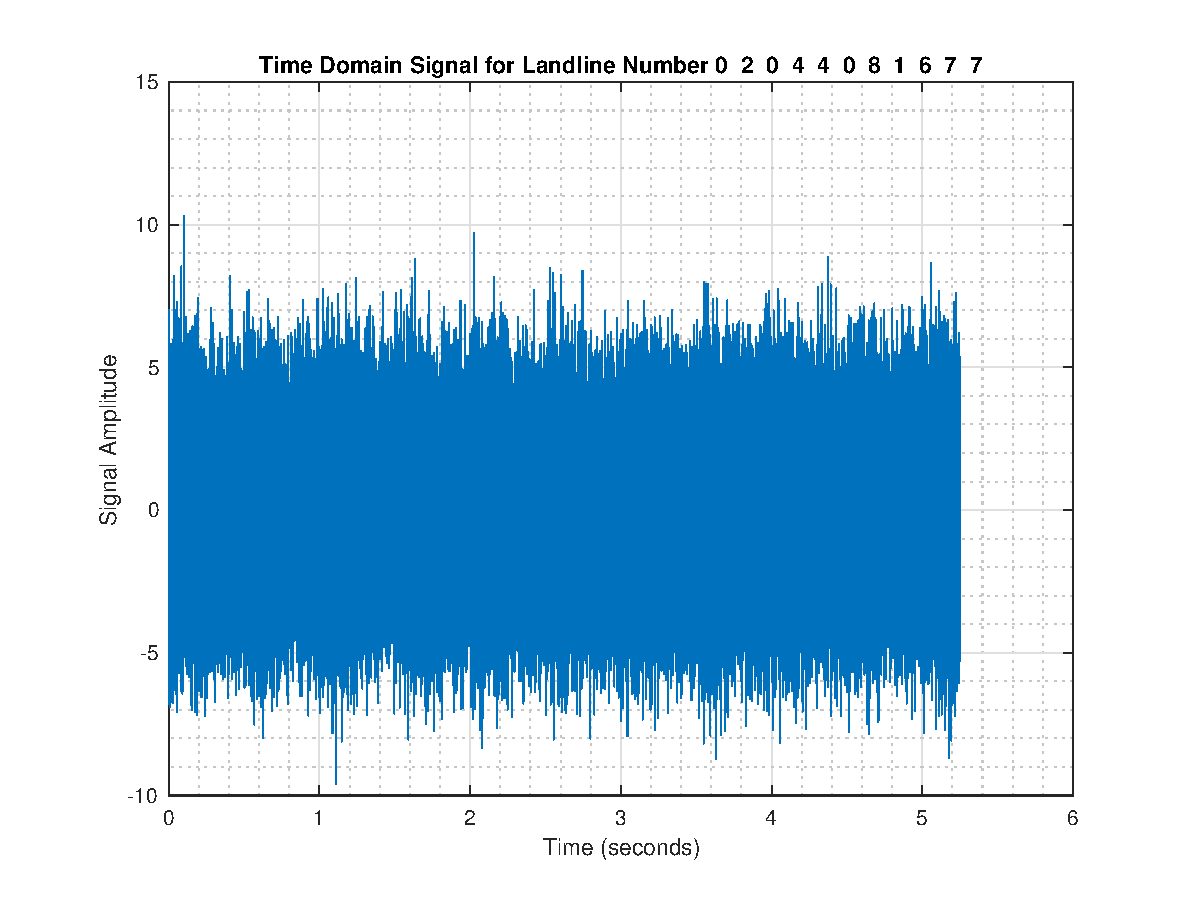
\includegraphics[width = \textwidth]{dtp_fullsig_n2}
\caption{Time domain, $\sigma_N=2$}
\label{fig:dtp_fullsig_n2}
\end{subfigure}
\begin{subfigure}{0.32\textwidth}
\centering
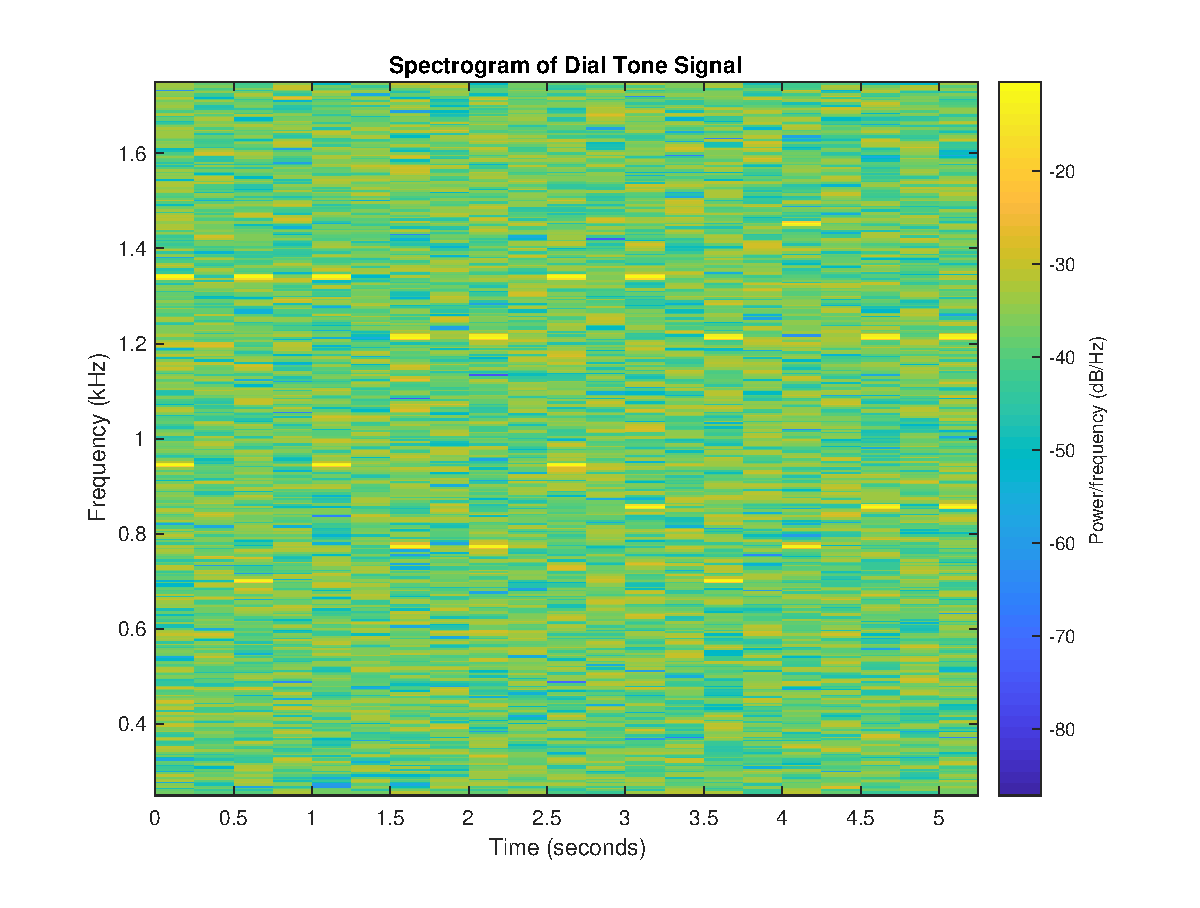
\includegraphics[width = \textwidth]{dtp_spec_n2}
\caption{Full spectrogram, $\sigma_N=2$}
\label{fig:dtp_spec_n2}
\end{subfigure}
\begin{subfigure}{0.32\textwidth}
\centering
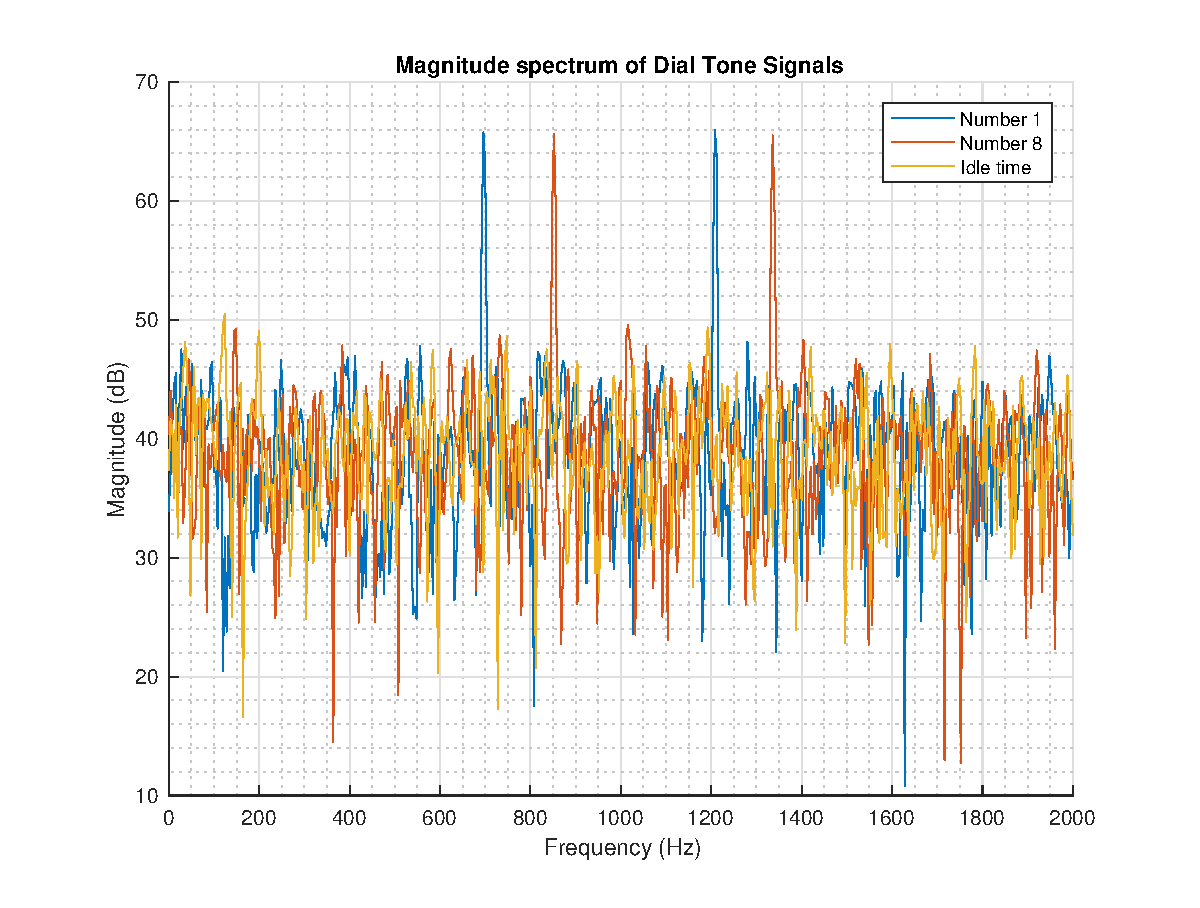
\includegraphics[width = \textwidth]{dtp_magspec_n2}
\caption{Power for digits 1 \& 8, $\sigma_N=2$}
\label{fig:dtp_magspec_n2}
\end{subfigure}
\begin{subfigure}{0.32\textwidth}
\centering
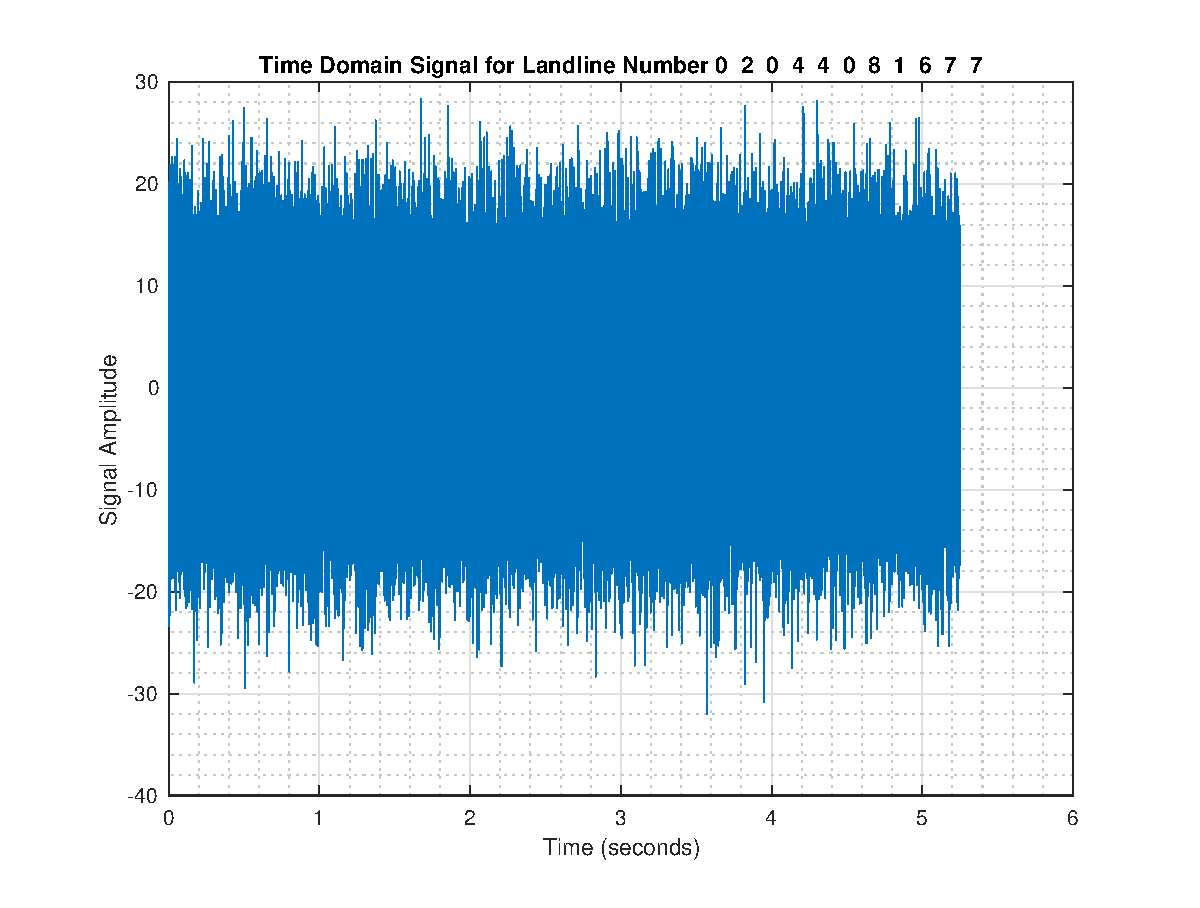
\includegraphics[width = \textwidth]{dtp_fullsig_n7}
\caption{Time domain, $\sigma_N=7$}
\label{fig:dtp_fullsig_n7}
\end{subfigure}
\begin{subfigure}{0.32\textwidth}
\centering
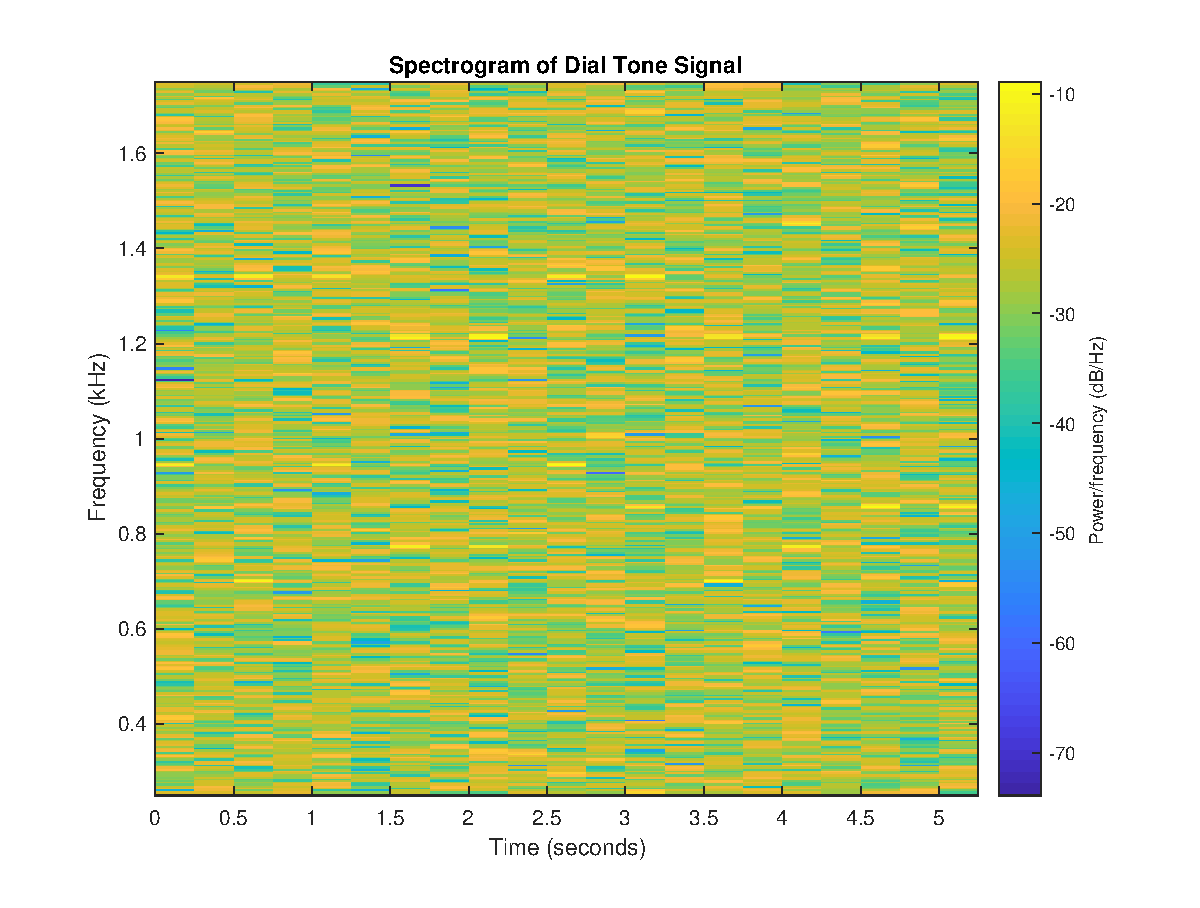
\includegraphics[width = \textwidth]{dtp_spec_n7}
\caption{Full spectrogram, $\sigma_N=7$}
\label{fig:dtp_spec_n7}
\end{subfigure}
\begin{subfigure}{0.32\textwidth}
\centering
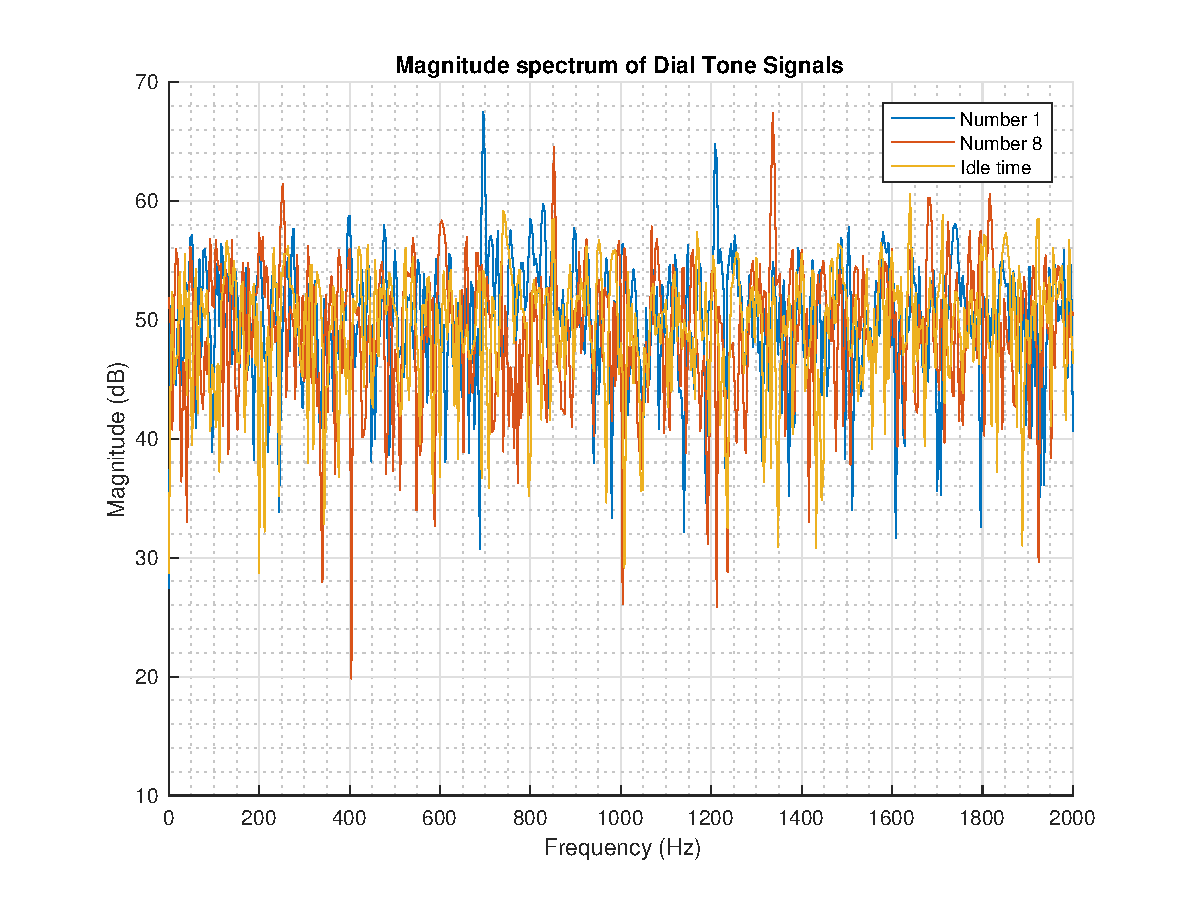
\includegraphics[width = \textwidth]{dtp_magspec_n7}
\caption{Power for digits 1 \& 8, $\sigma_N=7$}
\label{fig:dtp_magspec_n7}
\end{subfigure}
\begin{subfigure}{0.32\textwidth}
\centering
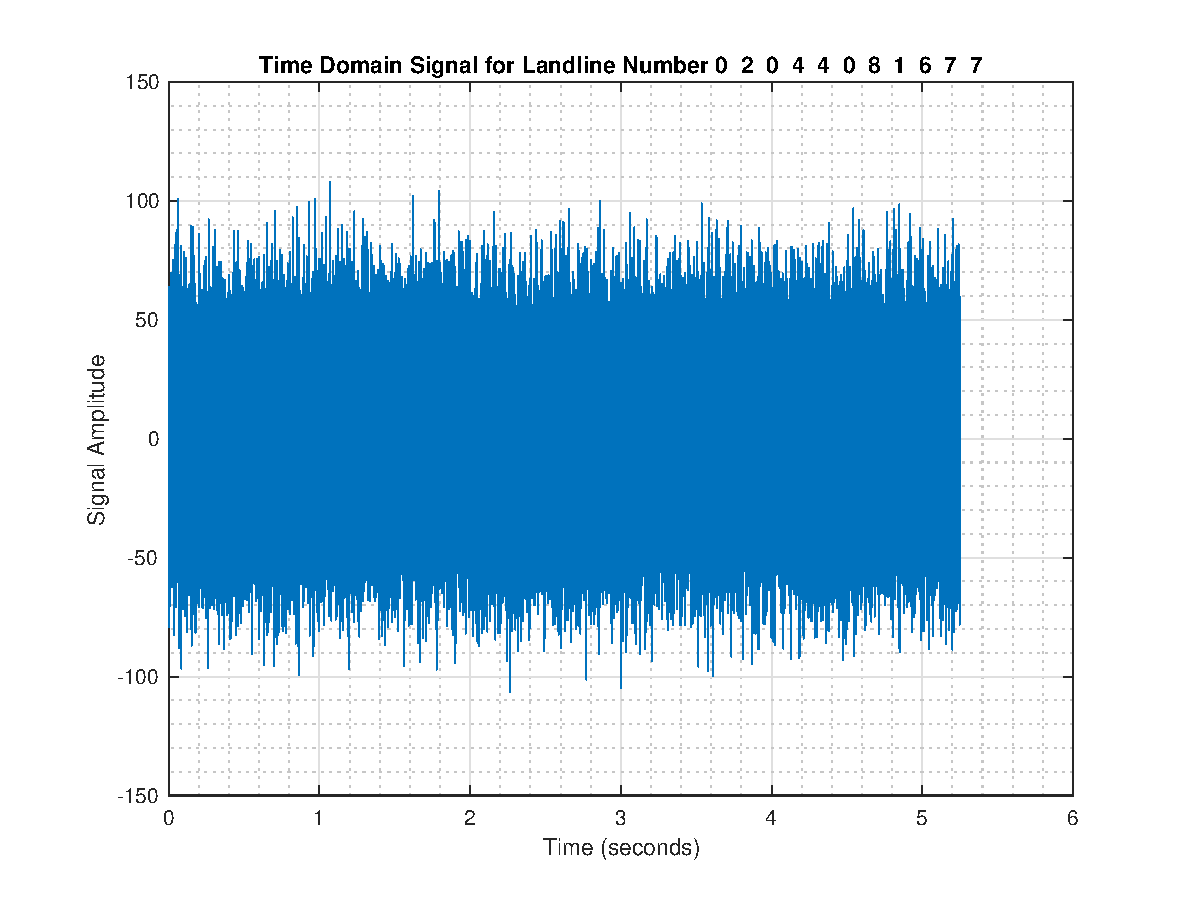
\includegraphics[width = \textwidth]{dtp_fullsig_n25}
\caption{Time domain, $\sigma_N=25$}
\label{fig:dtp_fullsig_n25}
\end{subfigure}
\begin{subfigure}{0.32\textwidth}
\centering
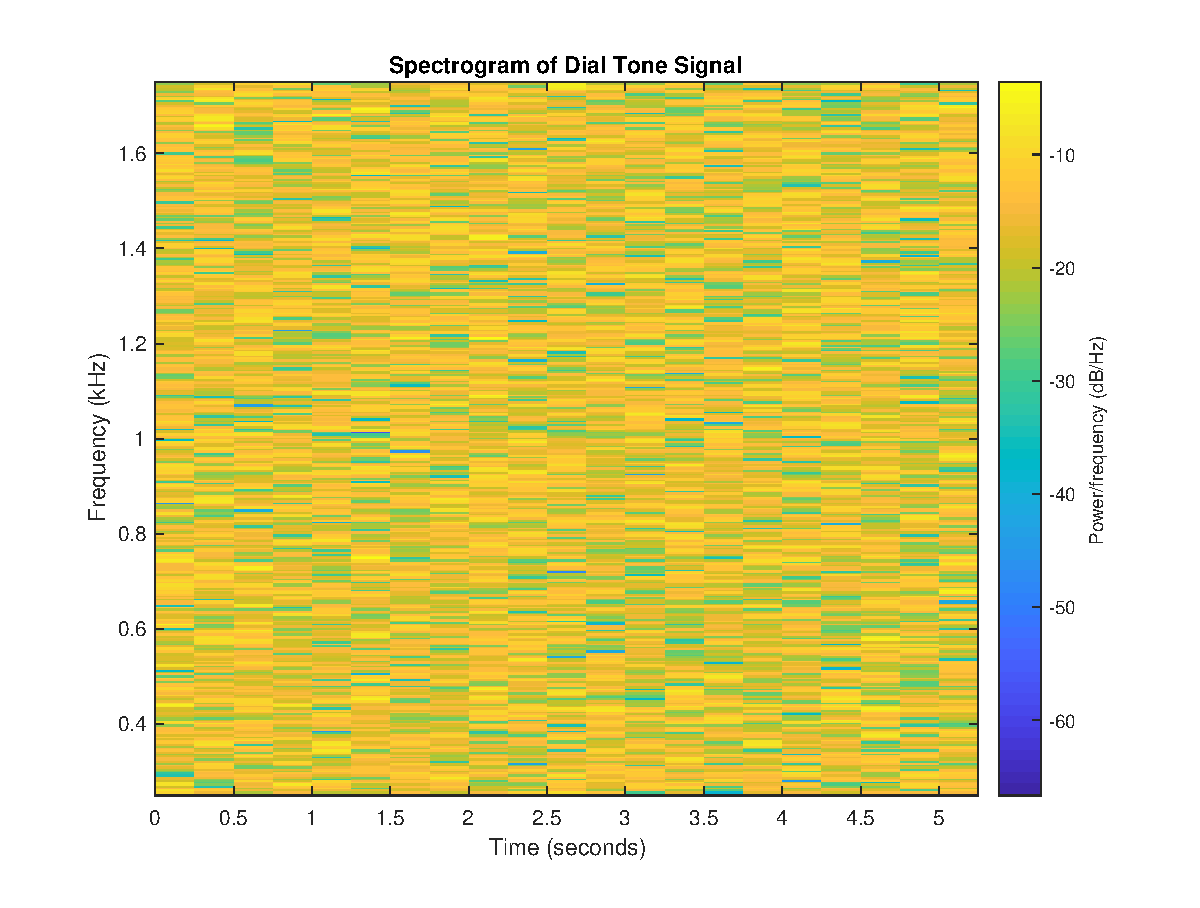
\includegraphics[width = \textwidth]{dtp_spec_n25}
\caption{Full spectrogram, $\sigma_N=25$}
\label{fig:dtp_spec_n25}
\end{subfigure}
\begin{subfigure}{0.32\textwidth}
\centering
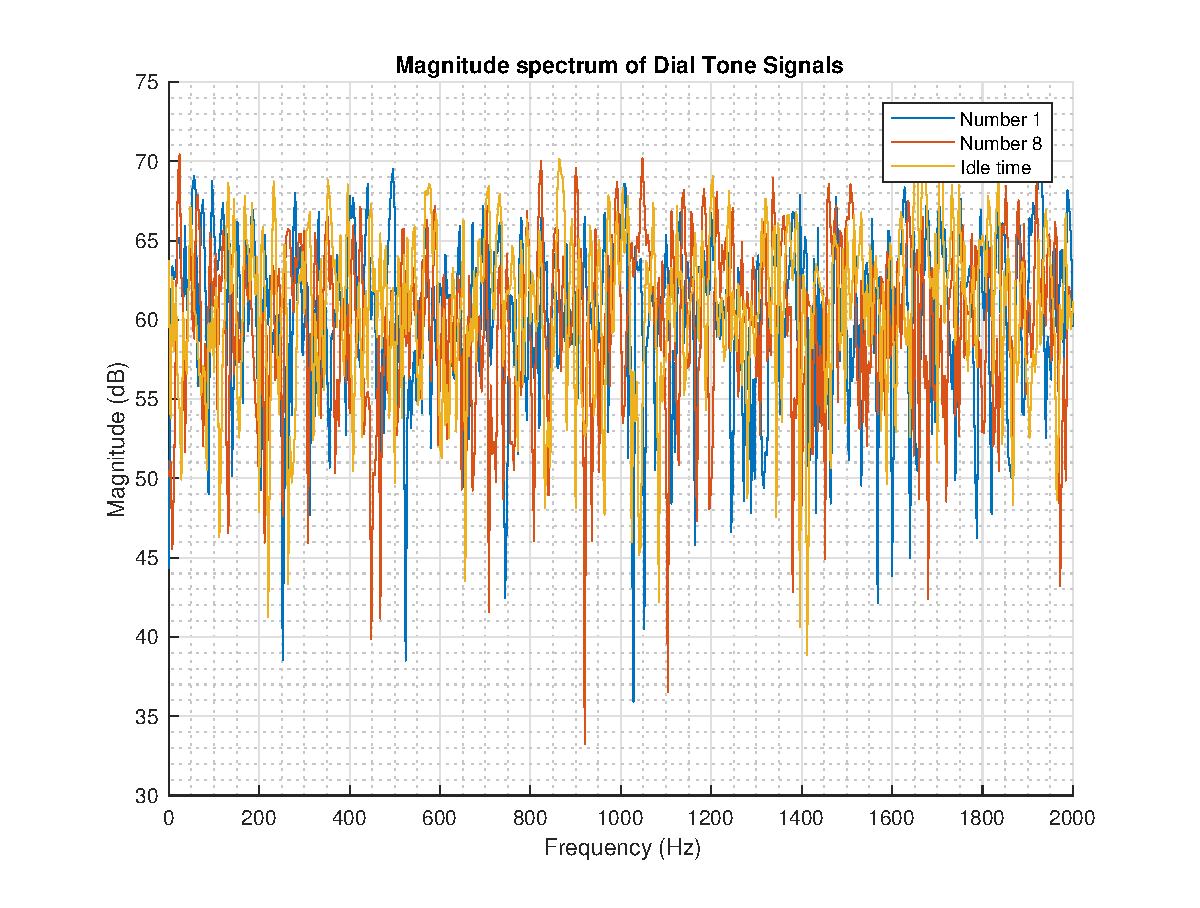
\includegraphics[width = \textwidth]{dtp_magspec_n25}
\caption{Power for digits 1 \& 8, $\sigma_N=25$}
\label{fig:dtp_magspec_n25}
\end{subfigure}
\caption{Comparing trends across the time domain signal and the spectrogram for numbers 1 and 8 for low, medium and high noise levels}
\label{spectrogram}
\end{figure}

\pagebreak

\subsection{Respiratory sinus arrhythmia from RR intervals}

Figure \ref{rr_pgm} shows the standard periodogram, an average periodogram with a 50 second window and an average periodogram with a 150 second window for all 3 trials.\\

A PSD spike indicates a high heart rate at the corresponding frequency, and the main difference between the 3 trials is the position of these peaks. Trial 1 involved normal breathing and therefore has a PSD peak at a higher frequency than Trial 2 and 3, which were for constrained breathing. Trial 3 induced a lower bpm (beats per minute) and hence has a peak at a larger frequency.\\

If we zoom into the average periodogram with a window of 50 seconds, we see that Trial 1 has a peak at a normalized frequency of 0.06 (with harmonics at 0.12), Trial 2 has a peak at 0.95 (with harmonics at 0.145 and 0.19), and Trial 3 has a peak at 0.16 (with harmonics at 0.25 and 0.33).

\begin{figure}[h!]
\centering
\begin{subfigure}{0.32\textwidth}
\centering
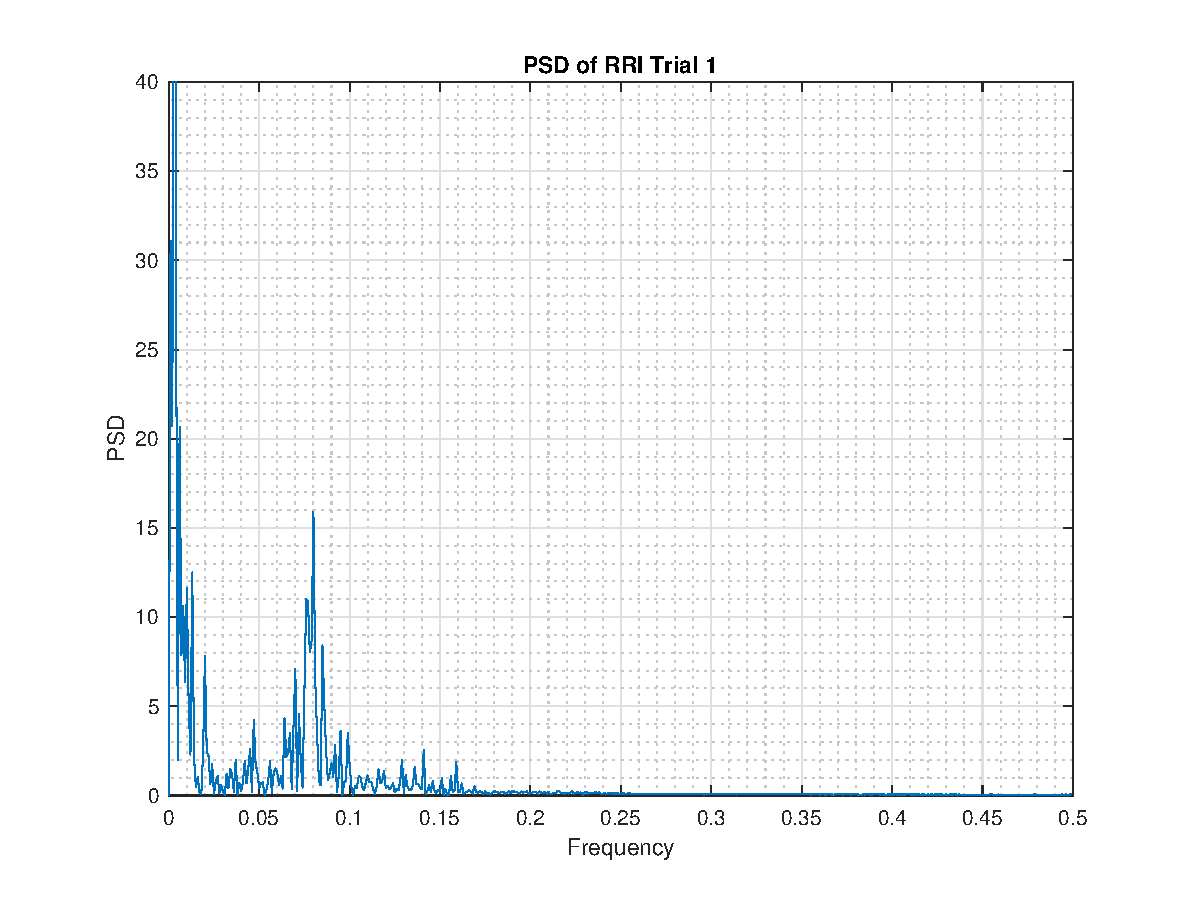
\includegraphics[width = \textwidth]{rr_t1}
\caption{Trial 1 periodogram}
\label{fig:rr_t1}
\end{subfigure}
\begin{subfigure}{0.32\textwidth}
\centering
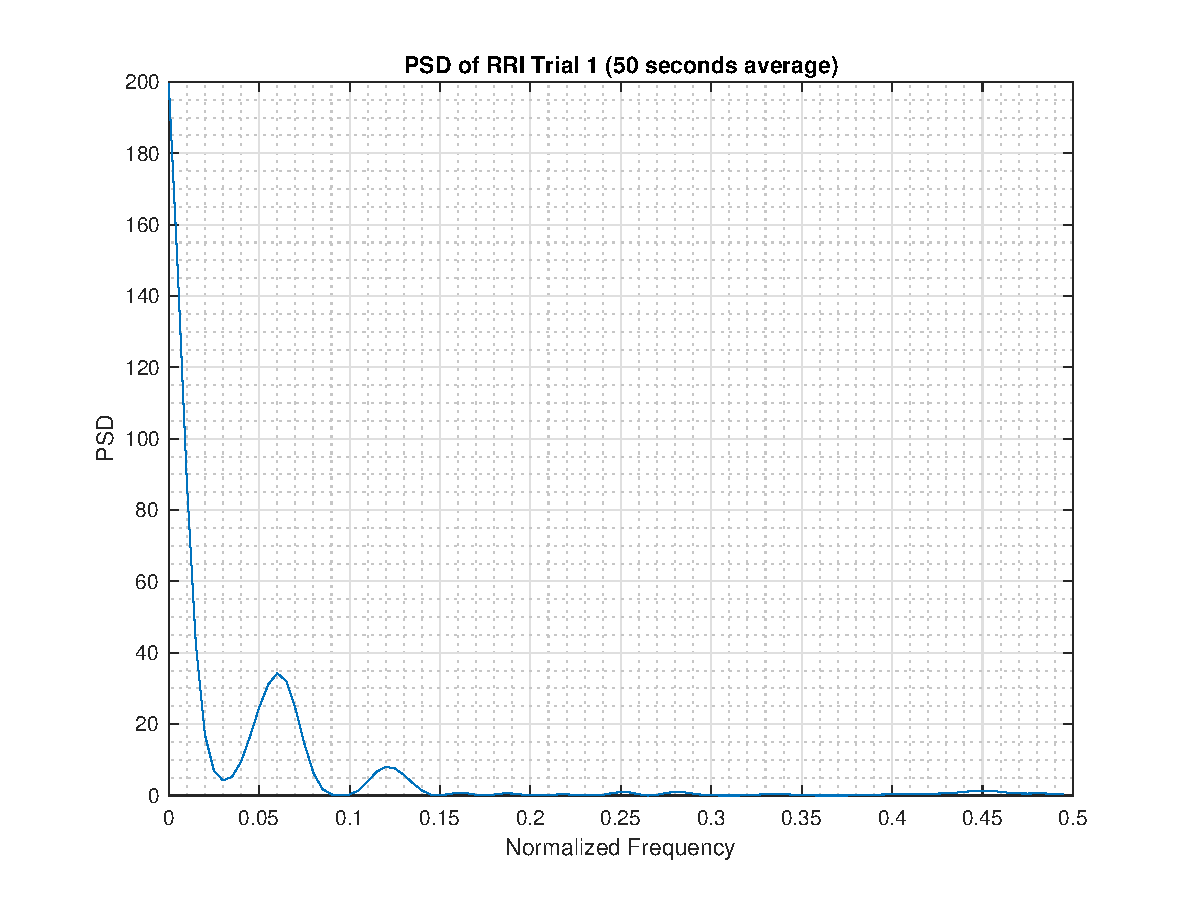
\includegraphics[width = \textwidth]{rr_t1_50}
\caption{T1 avg periodogram (50 secs)}
\label{fig:rr_t1_50}
\end{subfigure}
\begin{subfigure}{0.32\textwidth}
\centering
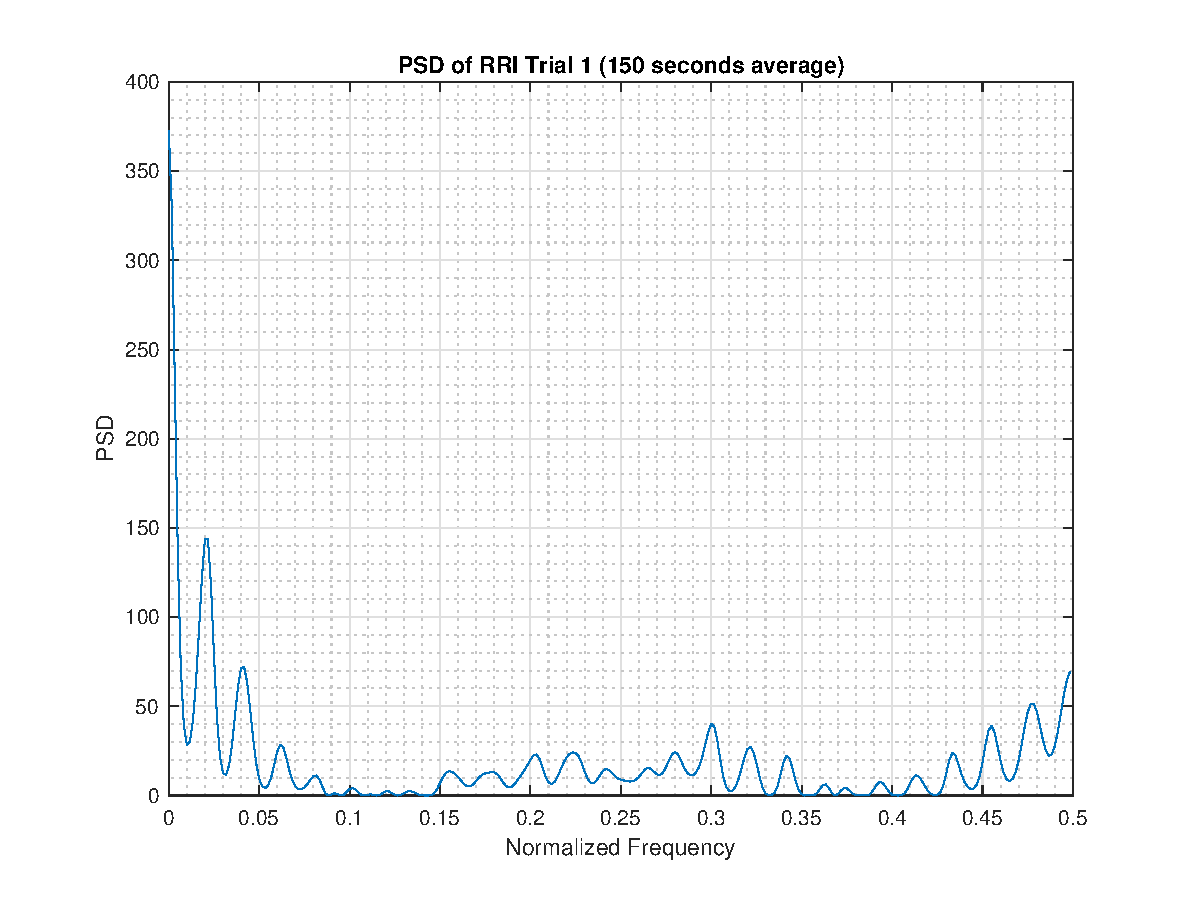
\includegraphics[width = \textwidth]{rr_t1_150}
\caption{T1 avg periodogram (150 secs)}
\label{fig:rr_t1_150}
\end{subfigure}
\begin{subfigure}{0.32\textwidth}
\centering
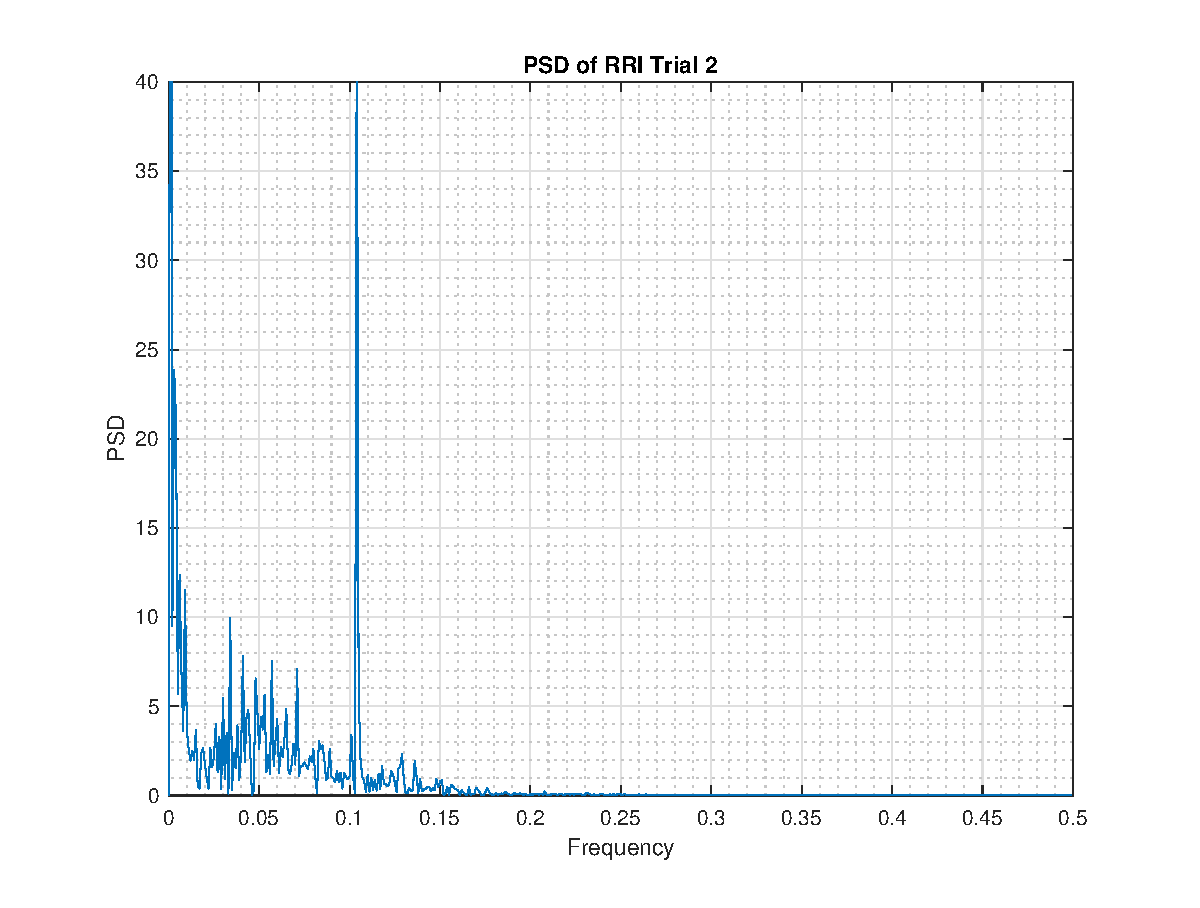
\includegraphics[width = \textwidth]{rr_t2}
\caption{Trial 2 periodogram}
\label{fig:rr_t2}
\end{subfigure}
\begin{subfigure}{0.32\textwidth}
\centering
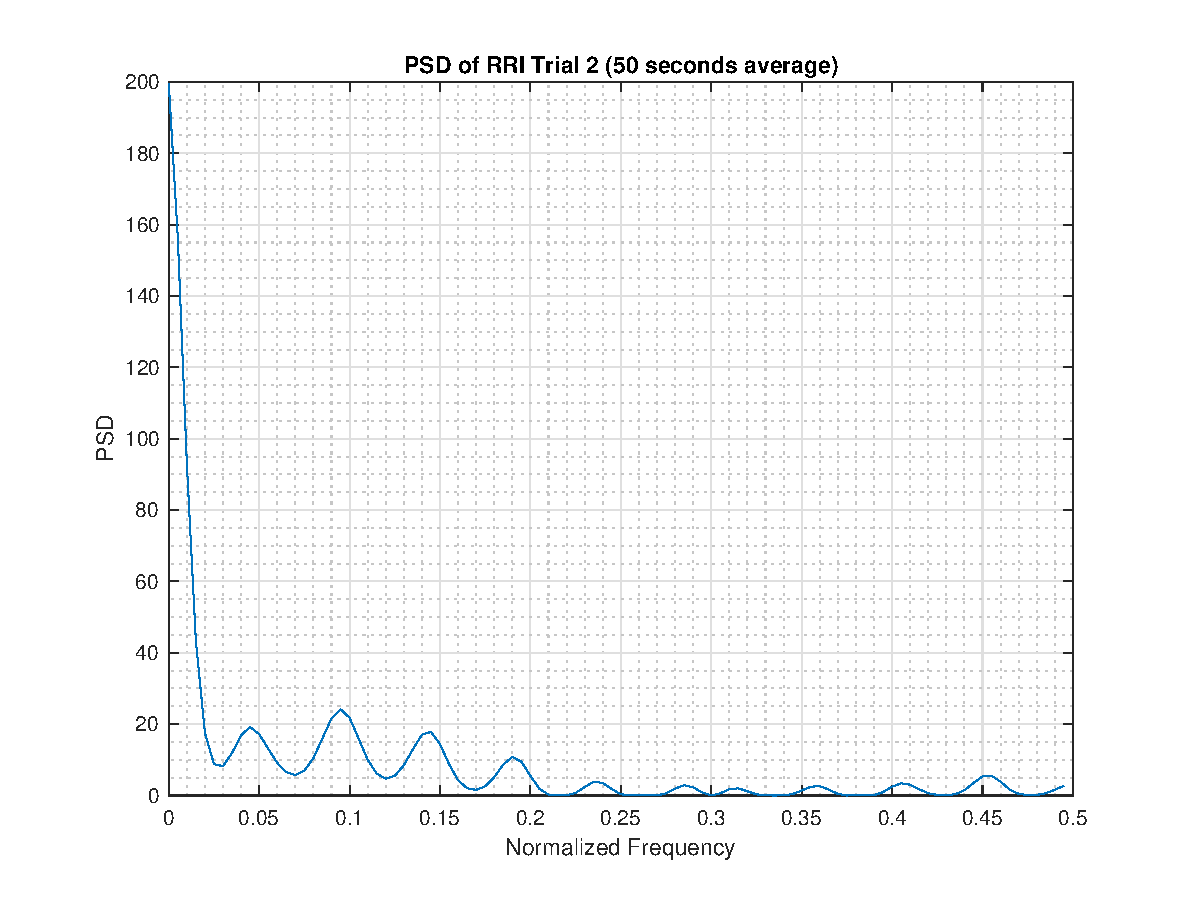
\includegraphics[width = \textwidth]{rr_t2_50}
\caption{T2 avg periodogram (50 secs)}
\label{fig:rr_t2_50}
\end{subfigure}
\begin{subfigure}{0.32\textwidth}
\centering
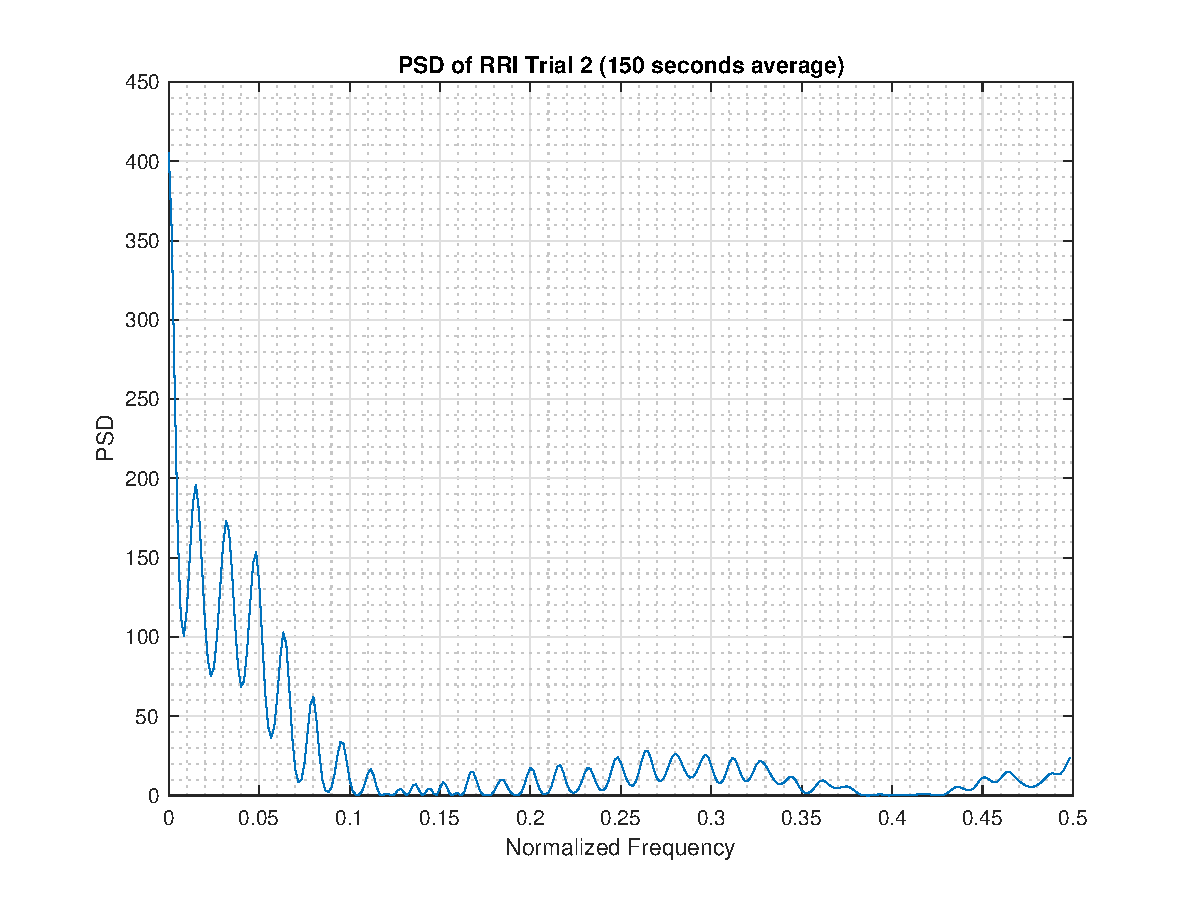
\includegraphics[width = \textwidth]{rr_t2_150}
\caption{T2 avg periodogram (150 secs)}
\label{fig:rr_t2_150}
\end{subfigure}
\begin{subfigure}{0.32\textwidth}
\centering
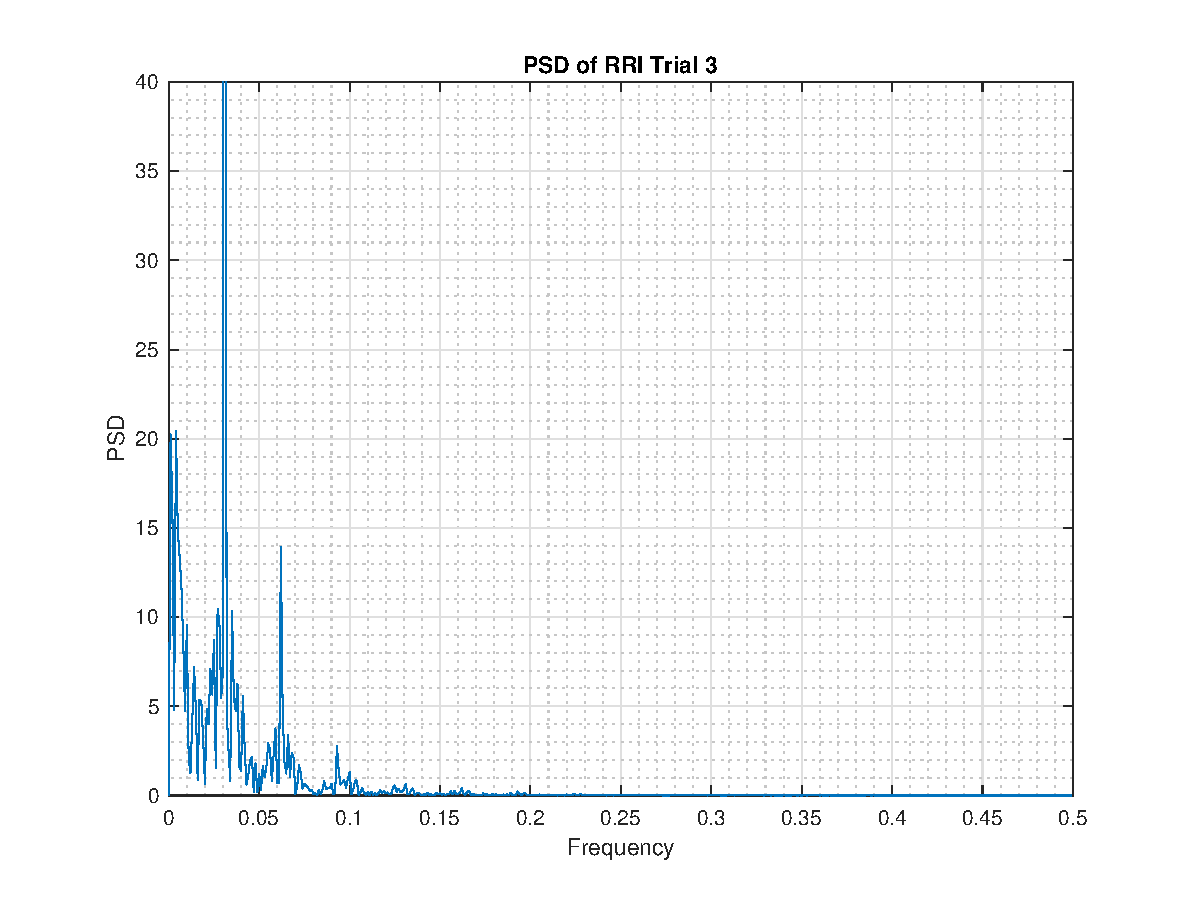
\includegraphics[width = \textwidth]{rr_t3}
\caption{Trial 3 periodogram}
\label{fig:rr_t3}
\end{subfigure}
\begin{subfigure}{0.32\textwidth}
\centering
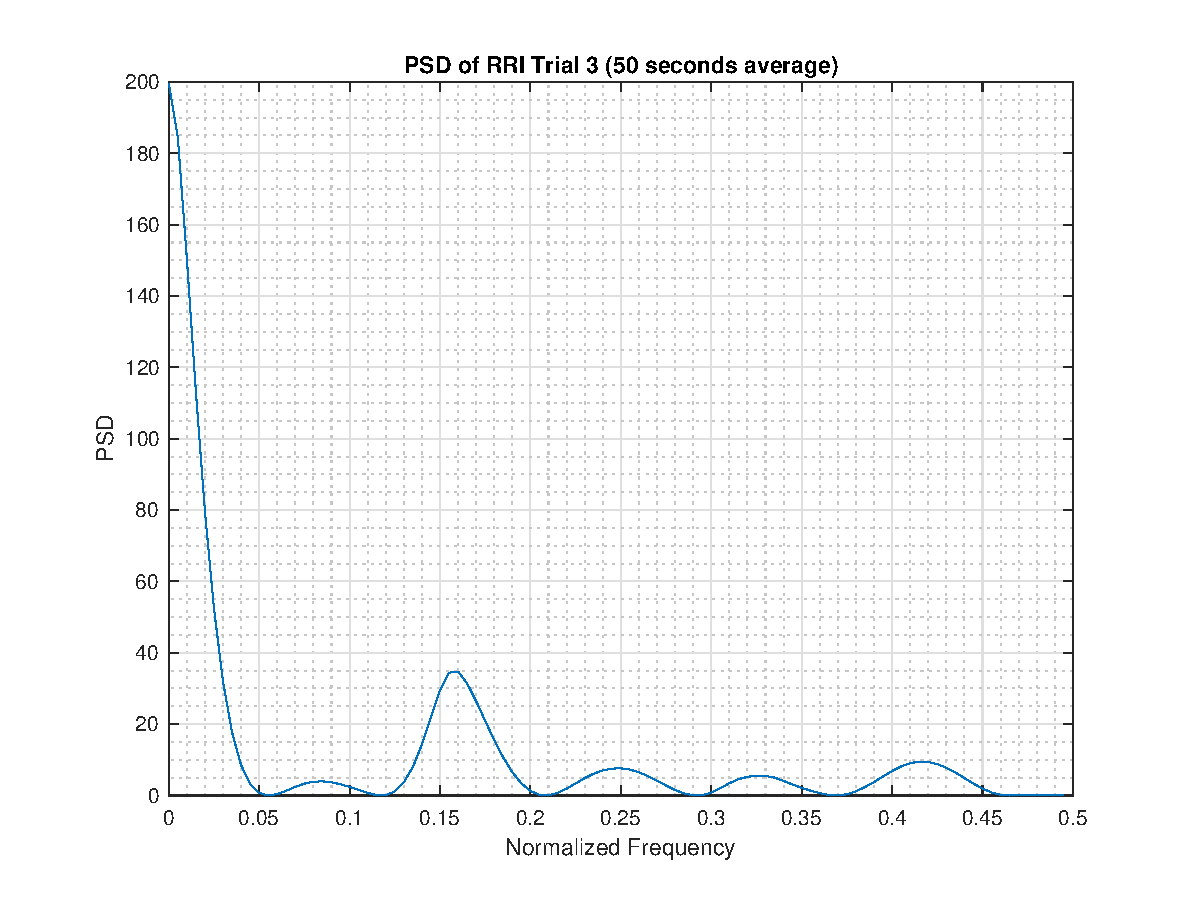
\includegraphics[width = \textwidth]{rr_t3_50}
\caption{T3 avg periodogram (50 secs)}
\label{fig:rr_t3_50}
\end{subfigure}
\begin{subfigure}{0.32\textwidth}
\centering
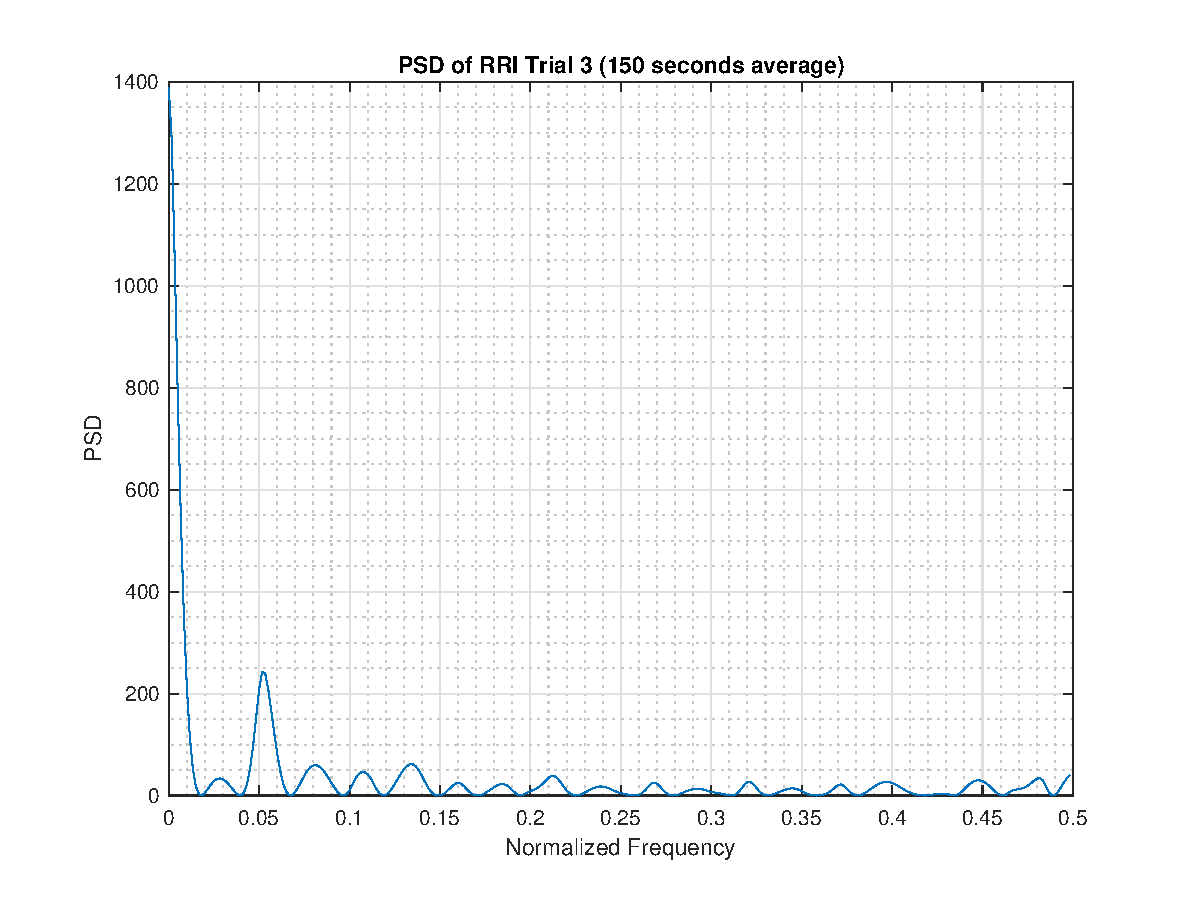
\includegraphics[width = \textwidth]{rr_t3_150}
\caption{T3 avg periodogram (150 secs)}
\label{fig:rr_t3_150}
\end{subfigure}
\caption{Comparing the PSD estimate for RRI Trials 1,2,3 from the standard periodogram, 50 second average periodogram and 150 second average periodogram}
\label{rr_pgm}
\end{figure}





\end{document}